\documentclass{article}
\usepackage{geometry}
\geometry{margin=0.8in}
%\documentclass[journal]{IEEEtran}
%\IEEEoverridecommandlockouts
\usepackage[utf8]{inputenc}
% The preceding line is only needed to identify funding in the first footnote. If that is unneeded, please comment it out.
\usepackage{cite}
\usepackage{amsmath,amssymb,amsfonts}
\usepackage{algorithmic}
\usepackage{graphicx}
\usepackage{float}
\usepackage{textcomp}
\usepackage{xcolor}
\usepackage{datetime}
\usepackage{tcolorbox}
\usepackage{varioref}
\restylefloat{table}
\usepackage{mathrsfs}
%\date{\displaydate{date}}

\usepackage{multicol}

\usepackage{tikz}
\usetikzlibrary{shapes,arrows}
\usepackage{verbatim}
%\usepackage[spanish]{babel}

\def\BibTeX{{\rm B\kern-.05em{\sc i\kern-.025em b}\kern-.08em
    T\kern-.1667em\lower.7ex\hbox{E}\kern-.125emX}}
    
\title{Control II\\
	\large Tarea 8. Control visual basado en imagen}
	
%\author{\IEEEauthorblockN{Marco Antonio Esquivel Basaldua}}
\author{Marco Antonio Esquivel Basaldua}
\begin{document}

\maketitle

	\section{Matriz de interacci\'on estimada en la posici\'on deseada}
	El estimar la matriz de interacci\'on solo a partir de la posici\'on deseada permite la realizaci\'on de menos c\'alculos al momento de llevar a cabo el control de la c\'amara. A continuaci\'on se presentan los resultados en MatLab, para un valor de longitud focal $f=0.002$, para los vectores de caracter\'isticas iniciales y deseadas siguientes.\newline
	
	\begin{center}
	\begin{multicols}{2}
	$$
	s_{init} = \left[\begin{matrix}
	-0.5\\0\\-0.8\\0^o\\0^o\\0^o
	\end{matrix}\right]
	$$
	$$
	s_{goal} = \left[\begin{matrix}
	0\\0\\-0.3\\0^o\\0^o\\0^o
	\end{matrix}\right]
	$$
	\end{multicols}
	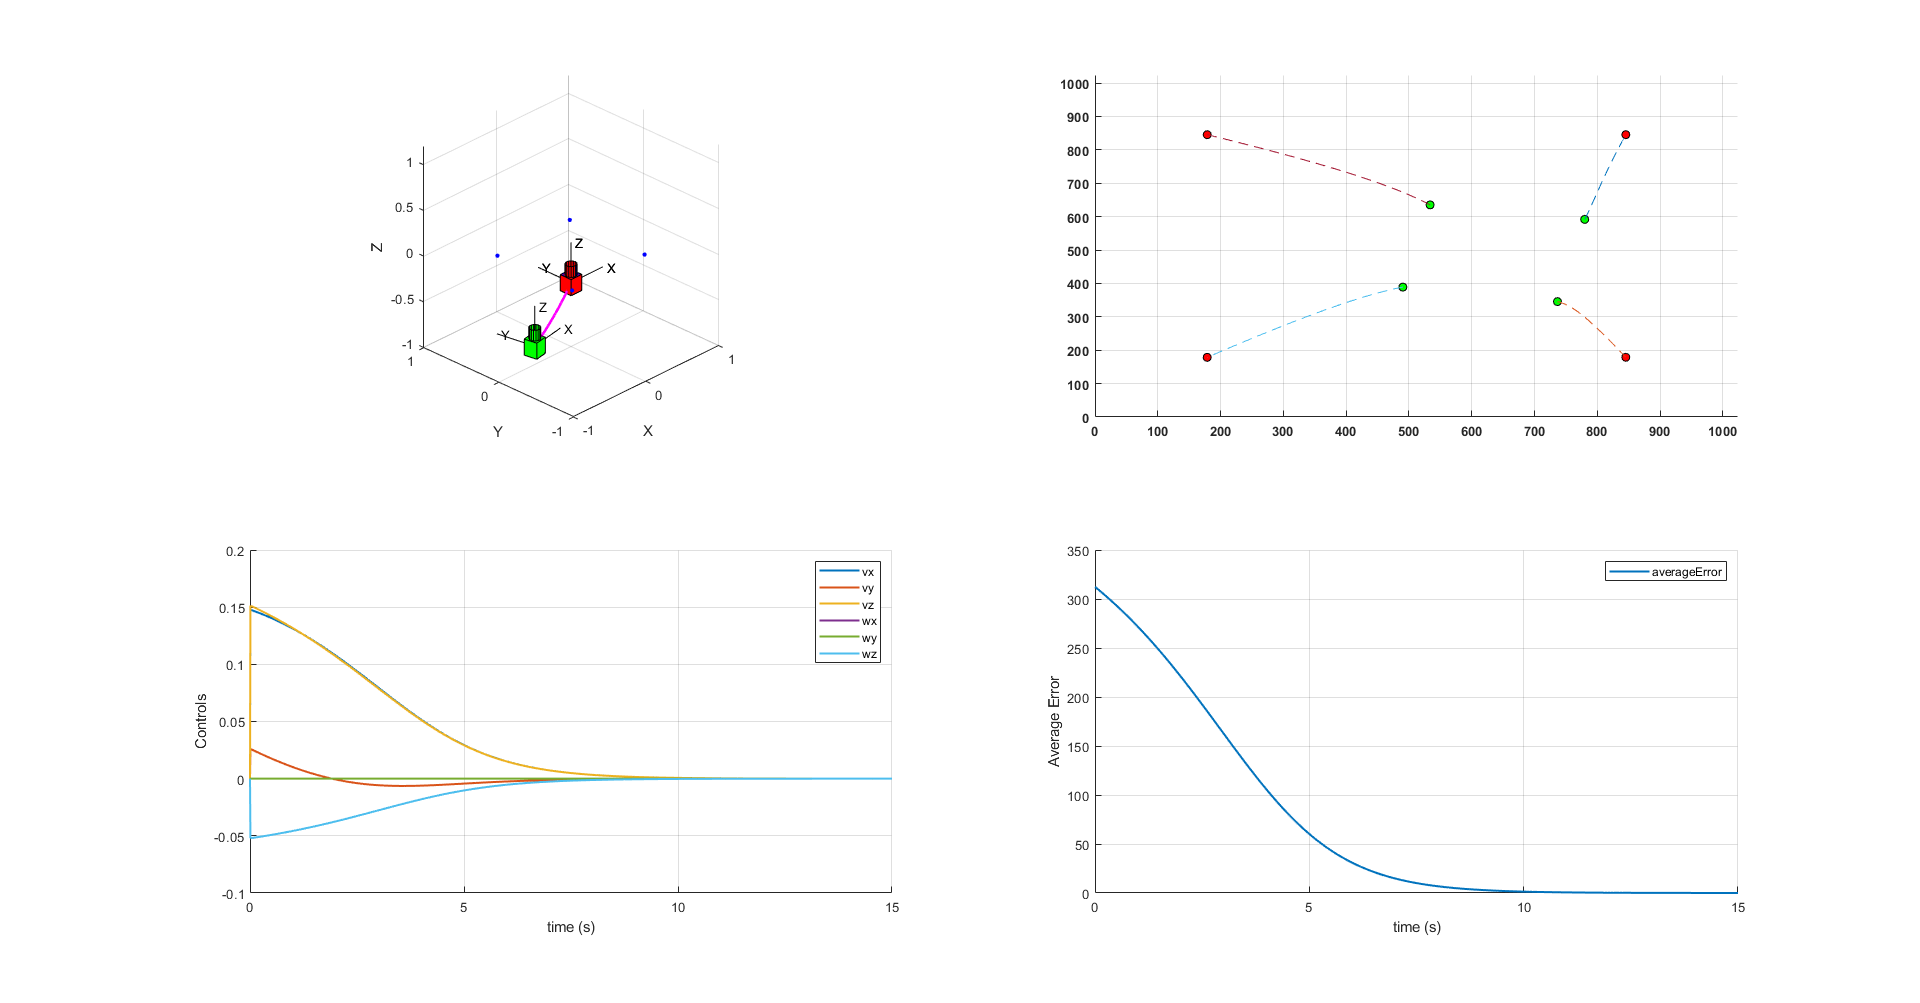
\includegraphics[scale=0.3]{fig2.png}\\
	{\footnotesize \textbf{Figura 1}. Comportamiento de los grados de libertad de la c\'amara. Se observa una convergencia exponencial a la posici\'on deseada.}
	\end{center}\newpage
	
	Para visualizar el comportamiento de la ley de control se proponen vectores de caracer\'isticas iniciales en las que solo una de las caracter\'isticas se ve afectada, es decir, una traslaci\'on a lo largo de uno solo de los ejes o una rotaci\'on sobre la misma. En todos los casos el vector de caracter\'isticas deseado es
	$$
	s = \left[\begin{matrix}
		0 & 0 &-0.6& 0^o& 0^o &0^o
	\end{matrix}\right]^\top
	$$
	\begin{center}
		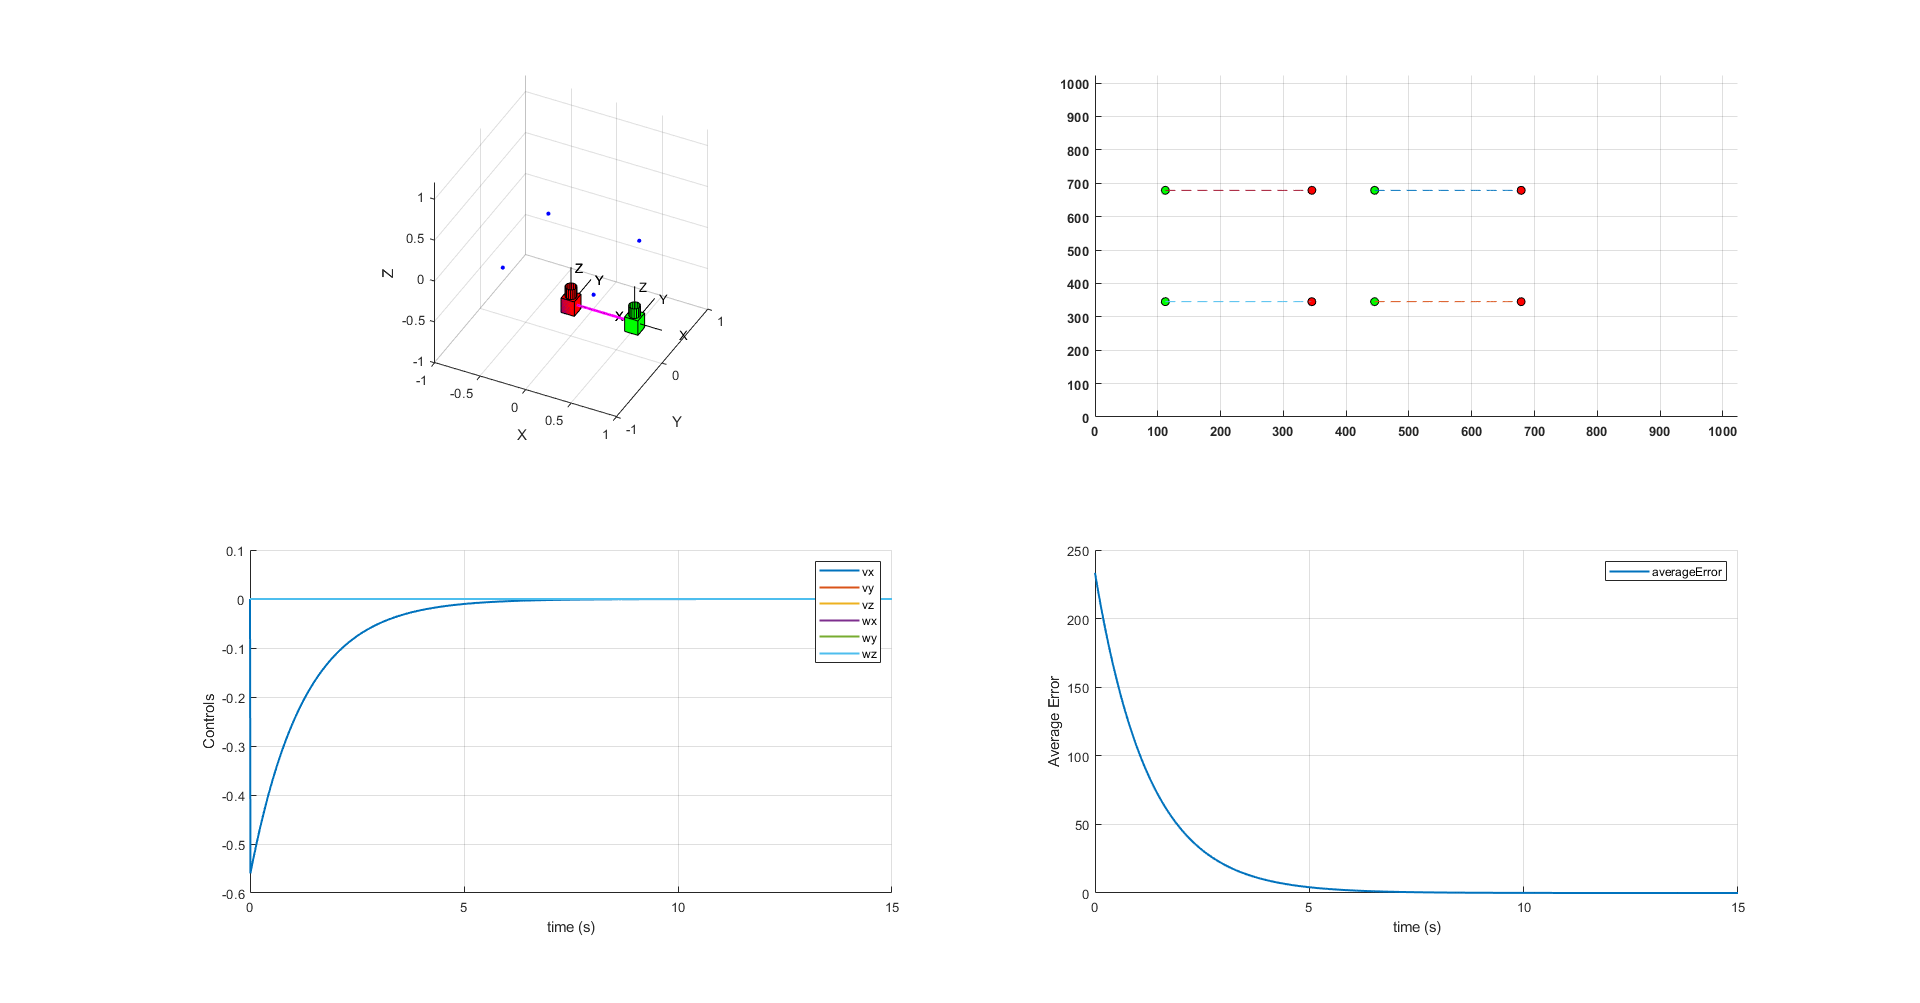
\includegraphics[scale=0.3]{extra_1.png}\\
	{\footnotesize \textbf{Figura 2}. Comportamiento de la ley de control a partir del vector de caracter\'isticas $s=[0.7,0,-0.6,0^o,0^o,0^o]$. La trayectoria de los puntos representa una linea recta que avanza en la imagen en el sentido contrario al movimeito de la c\'amara en e espacio 3D.}\\
	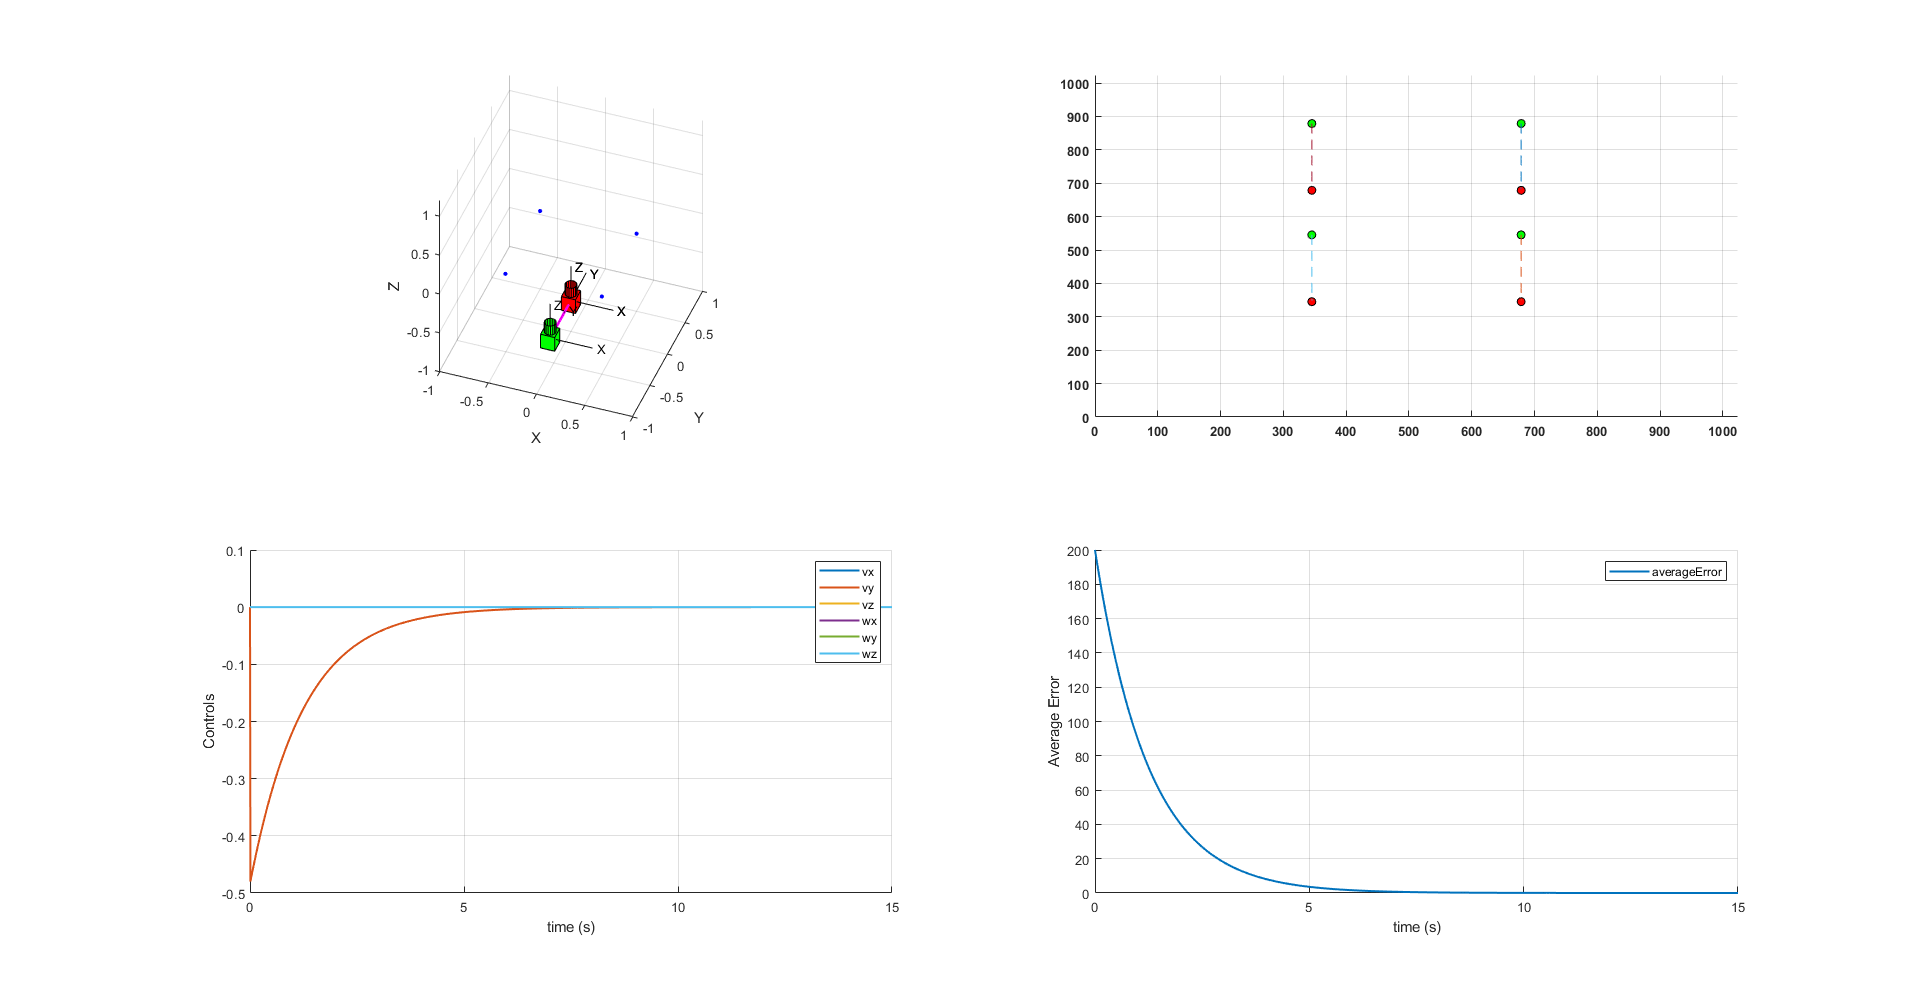
\includegraphics[scale=0.3]{extra_2.png}\\
	{\footnotesize \textbf{Figura 3}. Comportamiento de la ley de control a partir del vector de caracter\'isticas $s=[0,0.6,-0.6,0^o,0^o,0^o]$. La trayectoria de los puntos representa una linea recta que avanza en la imagen en el sentido contrario al movimeito de la c\'amara en e espacio 3D.}\\
	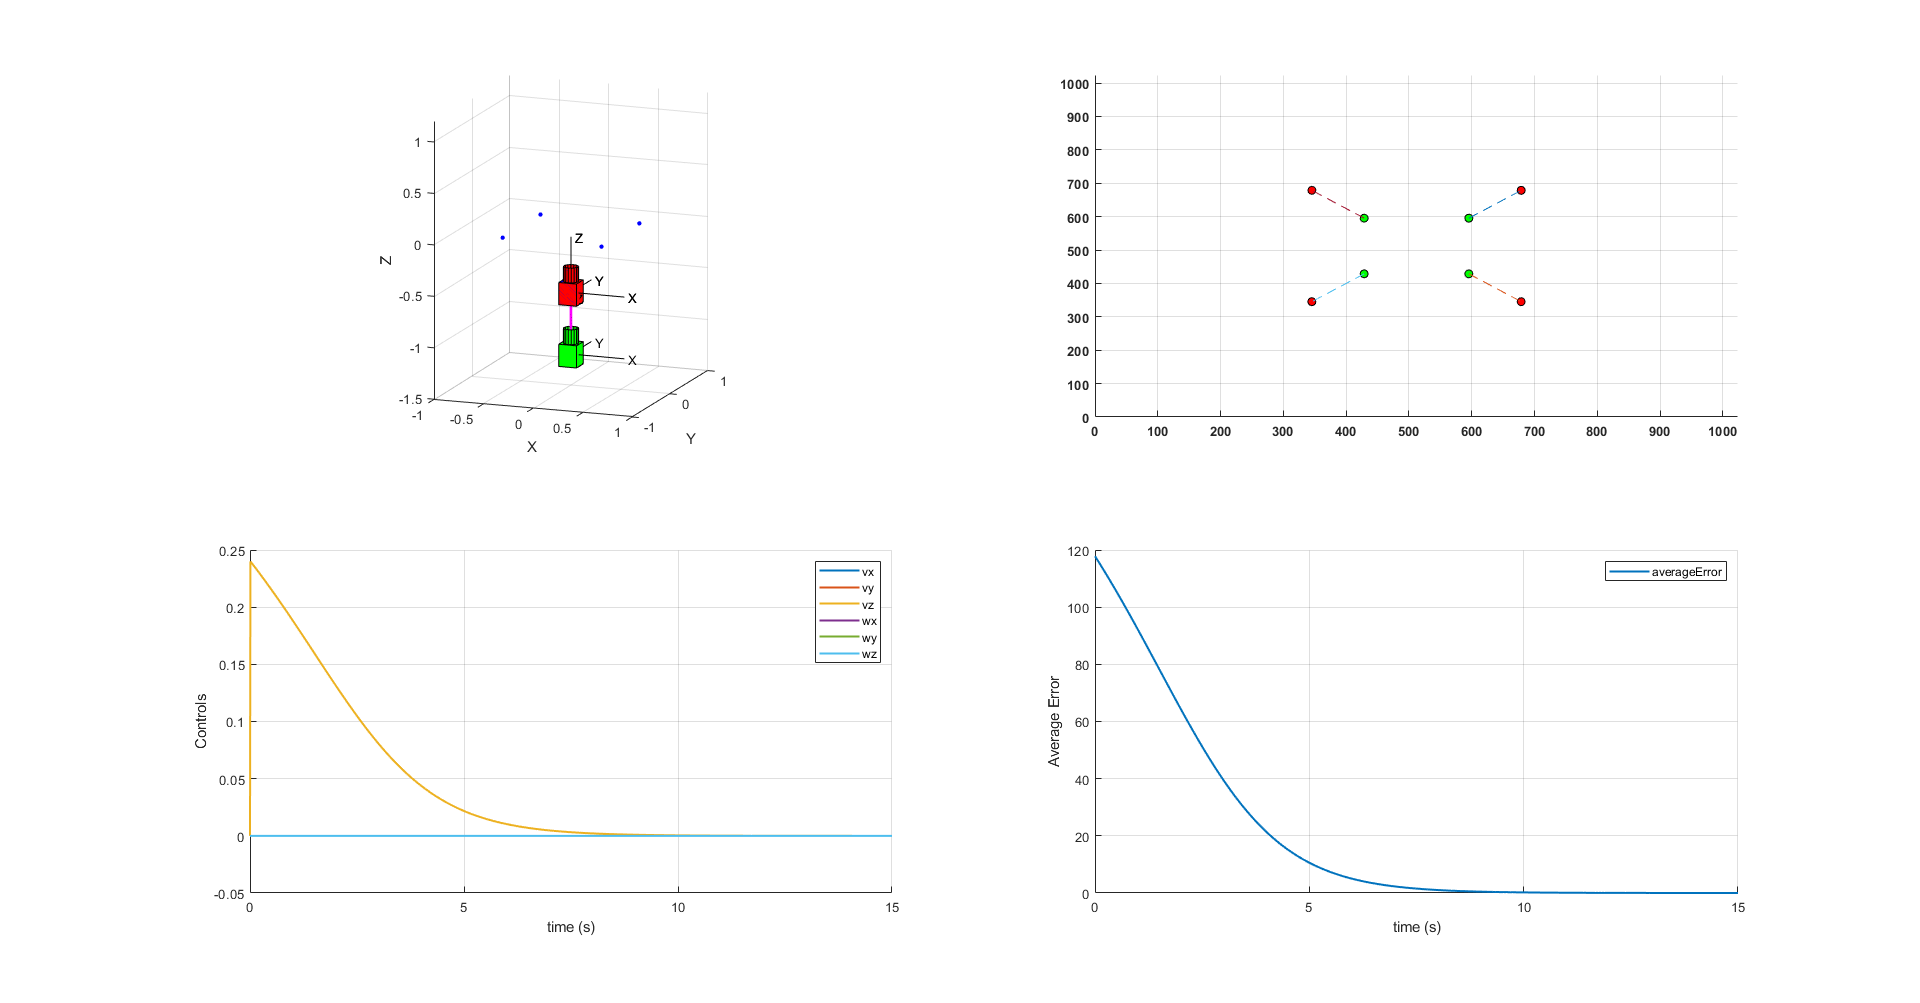
\includegraphics[scale=0.3]{extra_3.png}\\
	{\footnotesize \textbf{Figura 4}. Comportamiento de la ley de control a partir del vector de caracter\'isticas $s=[0,0,-1.2,0^o,0^o,0^o]$. Los puntos en la imagen se abren hacia los extremos ya que la c\'amara se acerca a ellos.}\\
	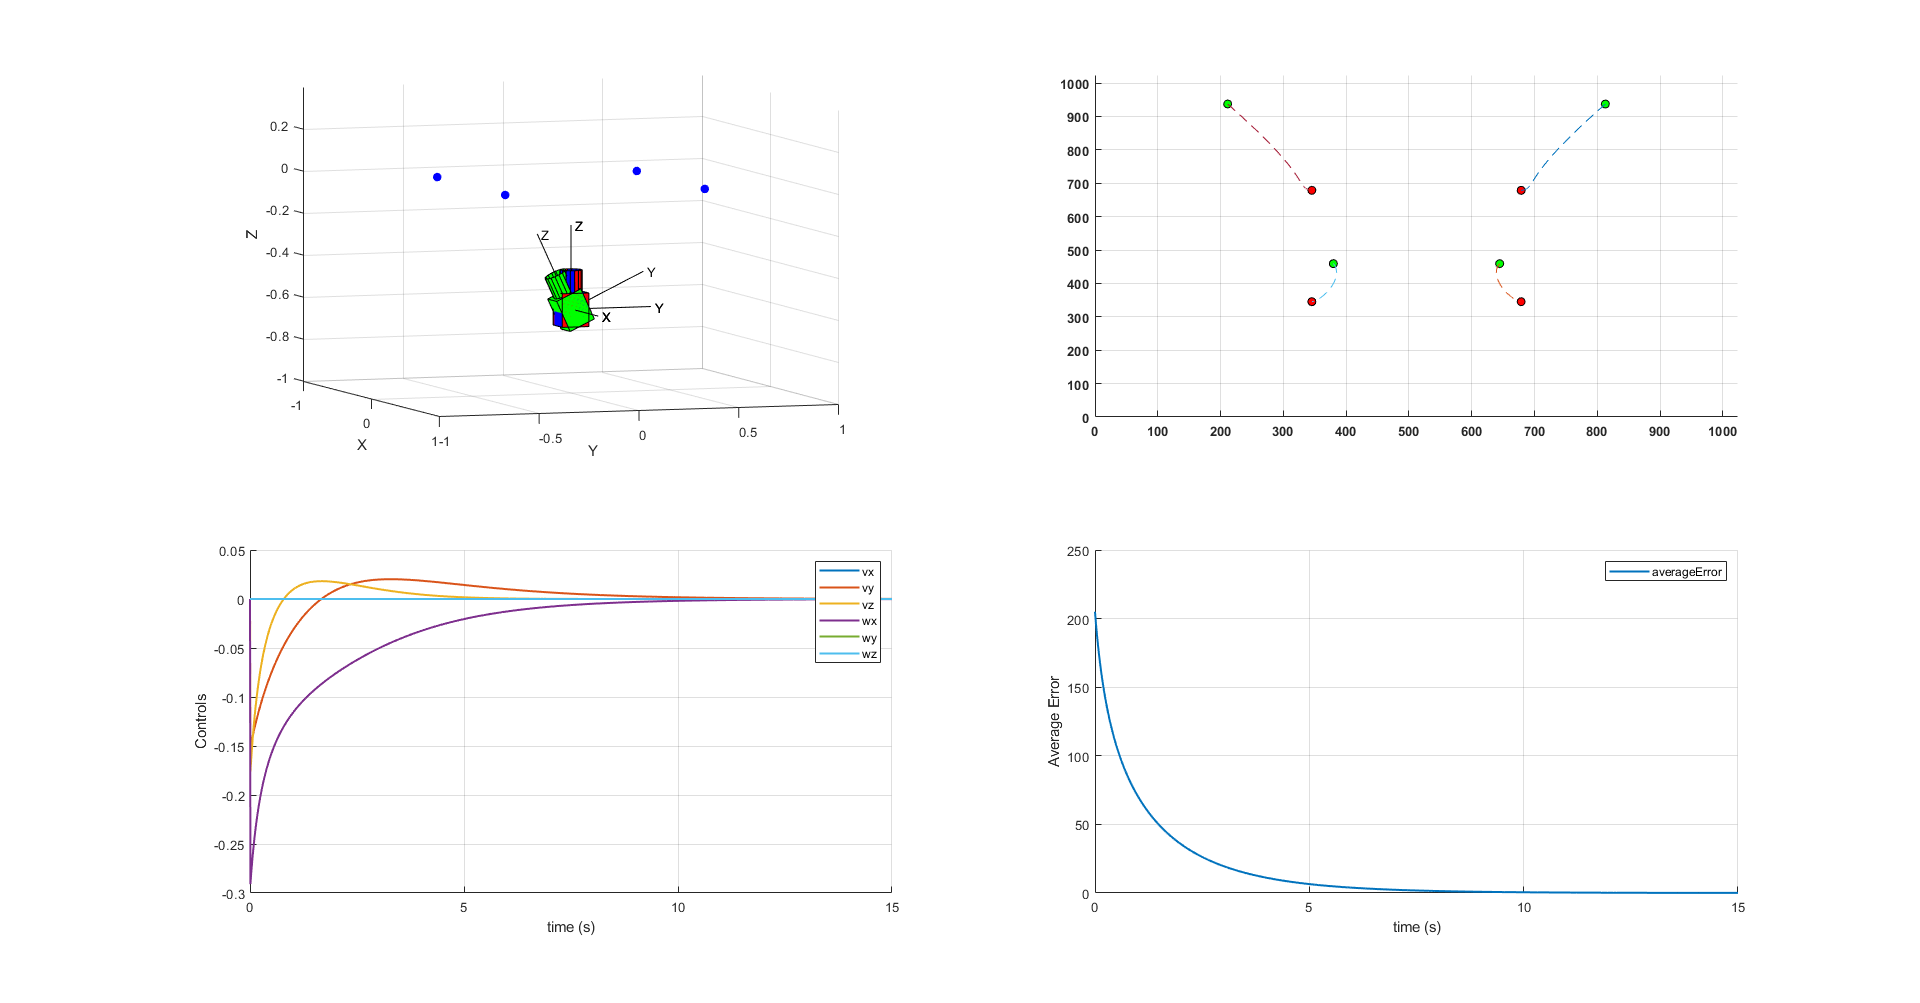
\includegraphics[scale=0.3]{extra_4.png}\\
	{\footnotesize \textbf{Figura 5}. Comportamiento de la ley de control a partir del vector de caracter\'isticas $s=[0,0,-0.6,25^o,0^o,0^o]$. Los puntos en la imagen describen un arco debido a la rotaci\'on de la c\'amara.}\\
	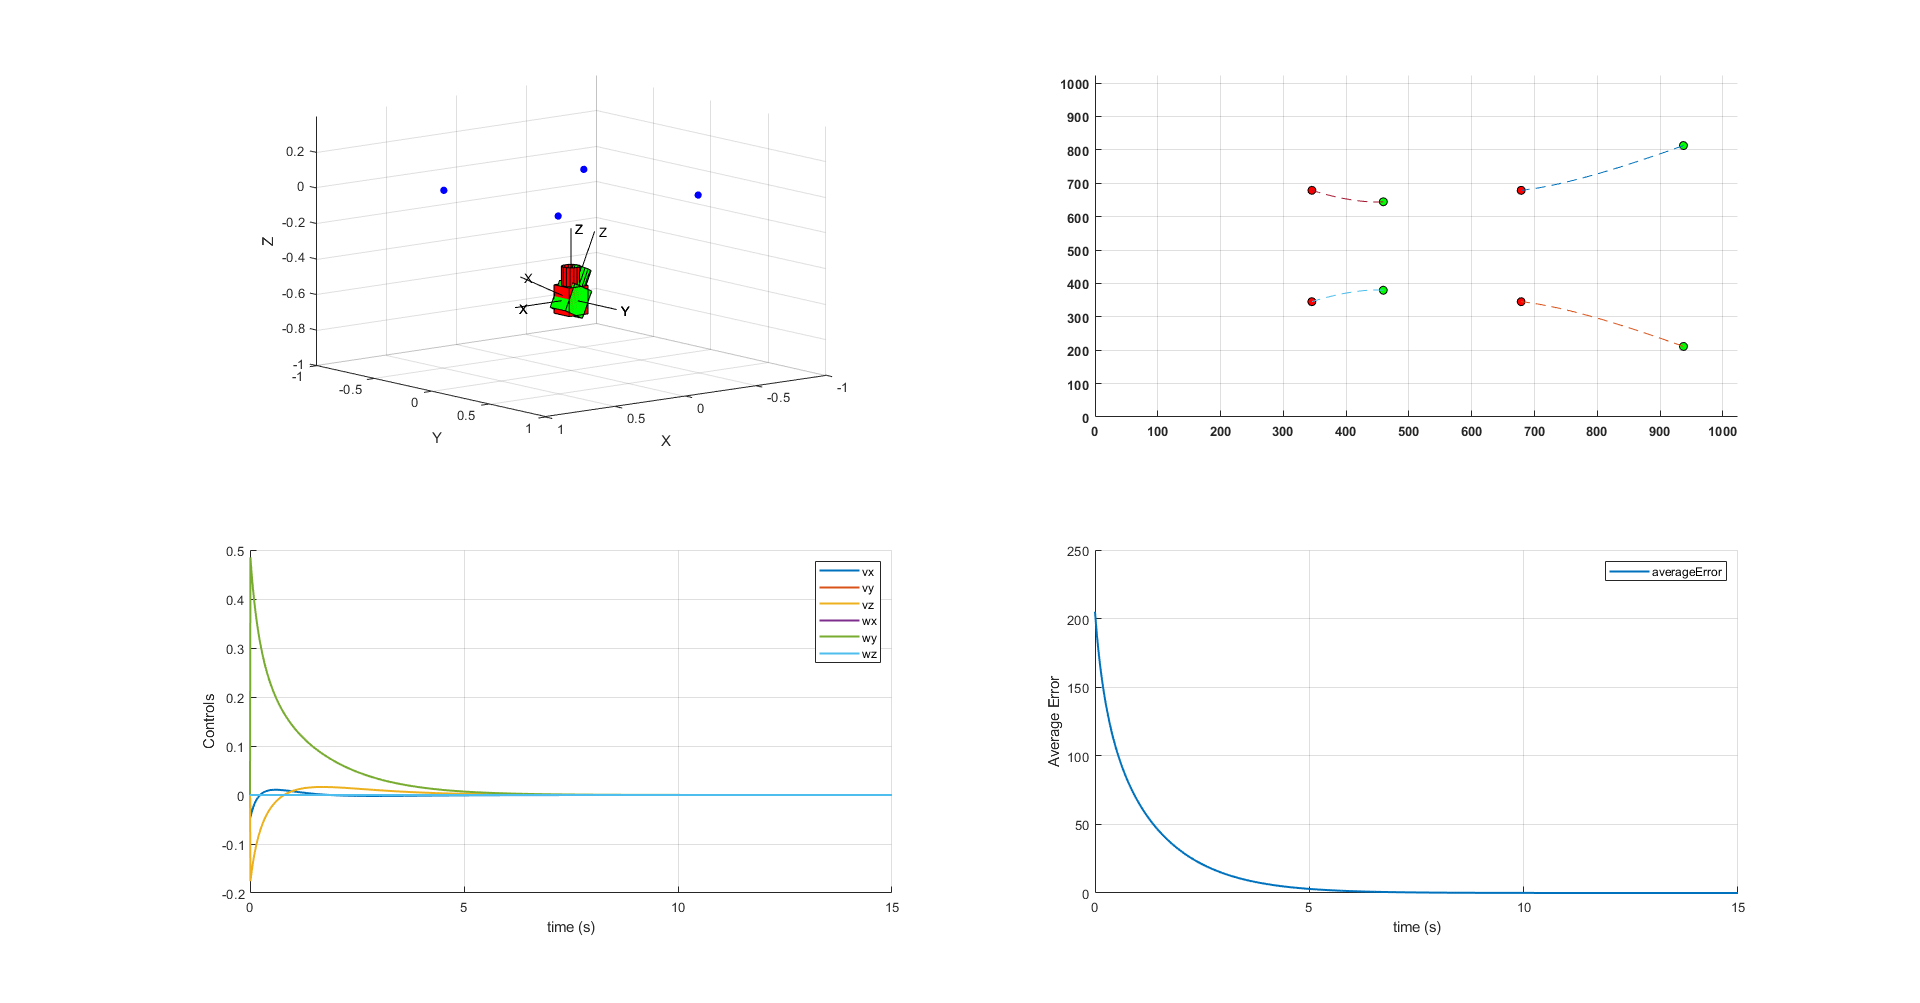
\includegraphics[scale=0.3]{extra_5.png}\\
	{\footnotesize \textbf{Figura 6}. Comportamiento de la ley de control a partir del vector de caracter\'isticas $s=[0,0,-0.6,0^o,-25^o,0^o]$. Los puntos en la imagen describen un arco debido a la rotaci\'on de la c\'amara.}\\
	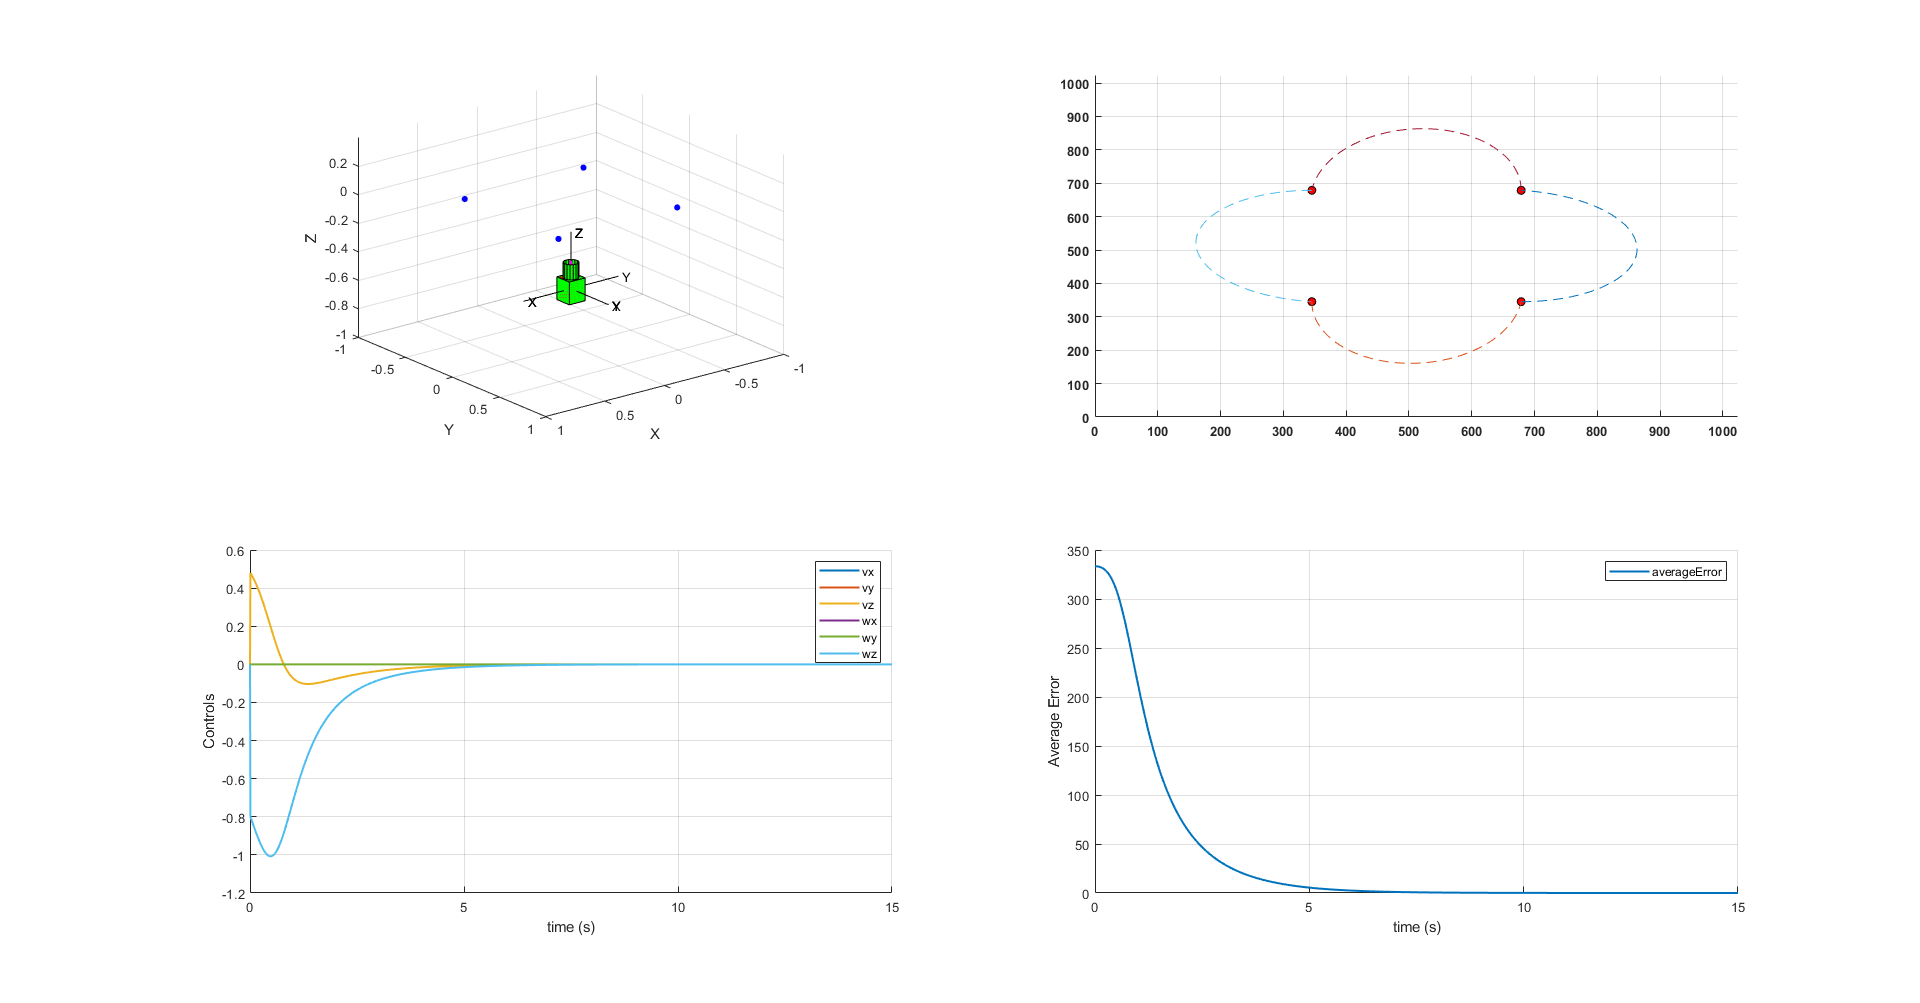
\includegraphics[scale=0.3]{extra_6.png}\\
	{\footnotesize \textbf{Figura 7}. Comportamiento de la ley de control a partir del vector de caracter\'isticas $s=[0,0,-0.6,0^o,0^o,90^o]$. La c\'amara solo hace una rotaci\'on sobre el eje $z$.}\\
	\end{center}
	
	Siguiendo usando este esquema, en el que la matriz de interacci\'on se calcula solamente a partir de la posici\'on deseada, se proponen dos movimientos generales, uno que comienza desde el vector de caracter\'isticas $s_1$ y otro a partir del vector $s_2$. En ambos movimientos se utiliza como vector de caracter\'isticas deseadas $s_{goal}$, el mismo usado en la figura 1.
	\begin{center}
	\begin{multicols}{2}
	$$
	s_{1} = \left[\begin{matrix}
	-0.5\\0\\-0.8\\-10^o\\30^o\\10^o
	\end{matrix}\right]
	$$
	$$
	s_{2} = \left[\begin{matrix}
	0.3\\0.8\\-0.9\\30^o\\10^o\\40^o
	\end{matrix}\right]
	$$
	\end{multicols}
	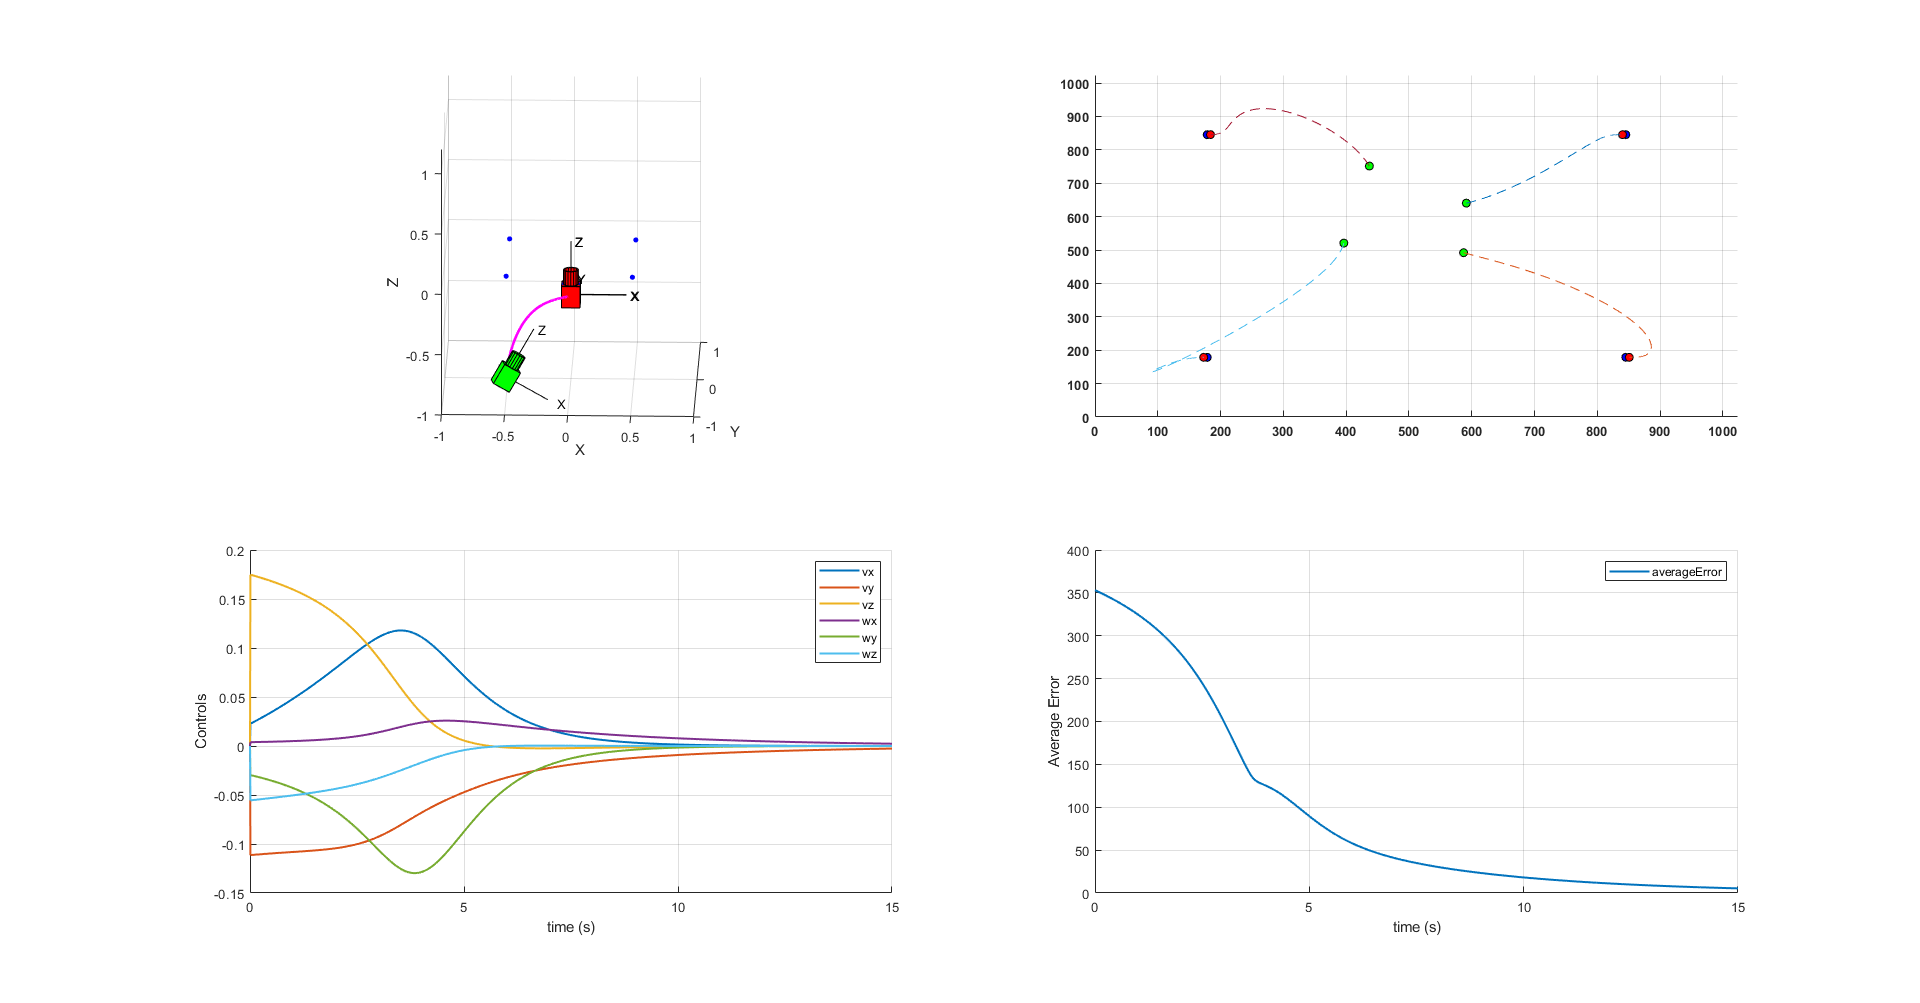
\includegraphics[scale=0.3]{fig3_1.png}\\
	{\footnotesize \textbf{Figura 8}. Resultados obtenidos a partir del vector de caracter\'isticas $s_1$. El comportamiento exponencial ocurre una vez que la c\'amara se encuentra cerca de la posici\'on deseada.}\\
	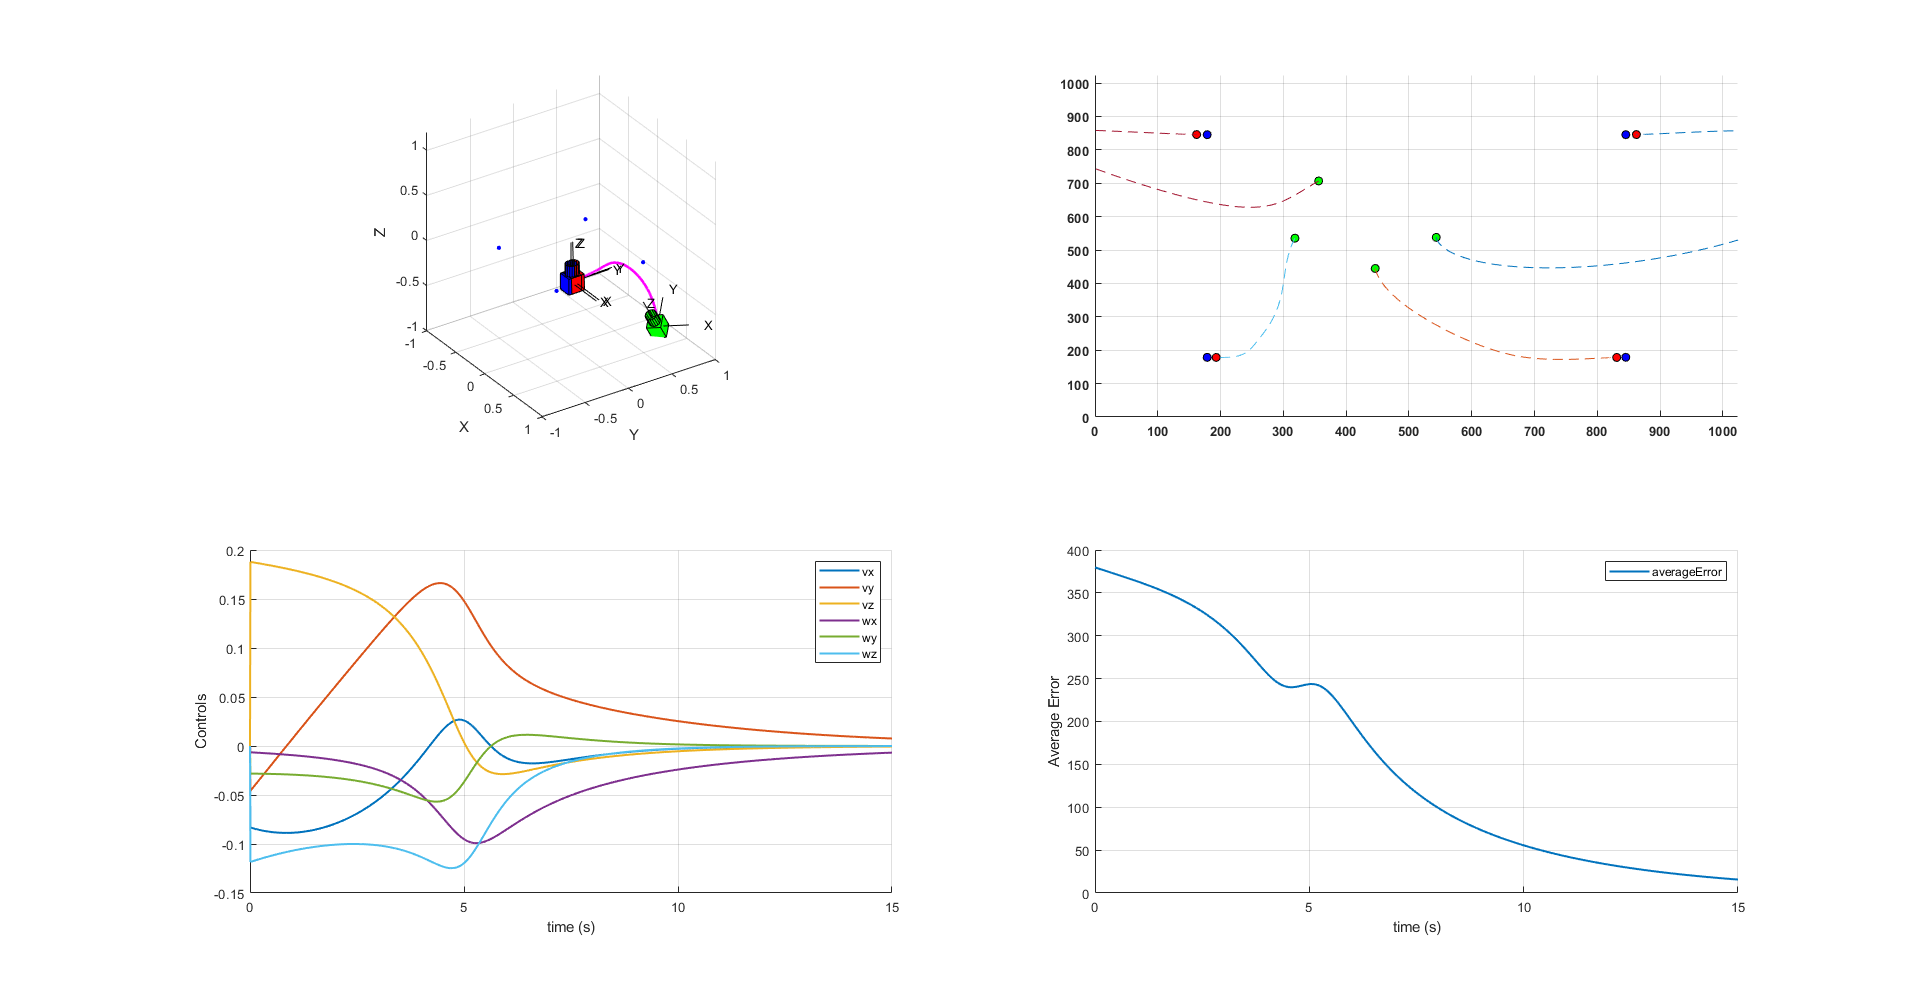
\includegraphics[scale=0.3]{fig3_2.png}\\
	{\footnotesize \textbf{Figura 9}. Resultados obtenidos a partir del vector de caracter\'isticas $s_2$. Al utilizar la matriz de interacci\'o c\'alculada solo a partir de la posici\'on deseada, la c\'amara hace que dos de los puntos salgan de la escena en la trayectoria a su posici\'on final. Nuevamente el comportamiento exponencial ocurre una vez que la c\'amara se encuentra cerca de la posici\'on deseada.}
	\end{center}\newpage
	
	\section{Subestimaci\'on, y sobreestimaci\'on de la profundidad de los puntos}
	Un par\'ametro importante es la estimaci\'on de la profundidad de los puntos. A continuaci\'on se presentan los resultados para una subestimaci\'on de esta profundidad, una estimaci\'on cercana a la real y una sobreestimaci\'on. Se utilizan los vectores de caracter\'isticas iniciales y deseadas $s_{init}$, $s_{goal}$ (mismos que en la figura 1).
	
	\begin{center}
	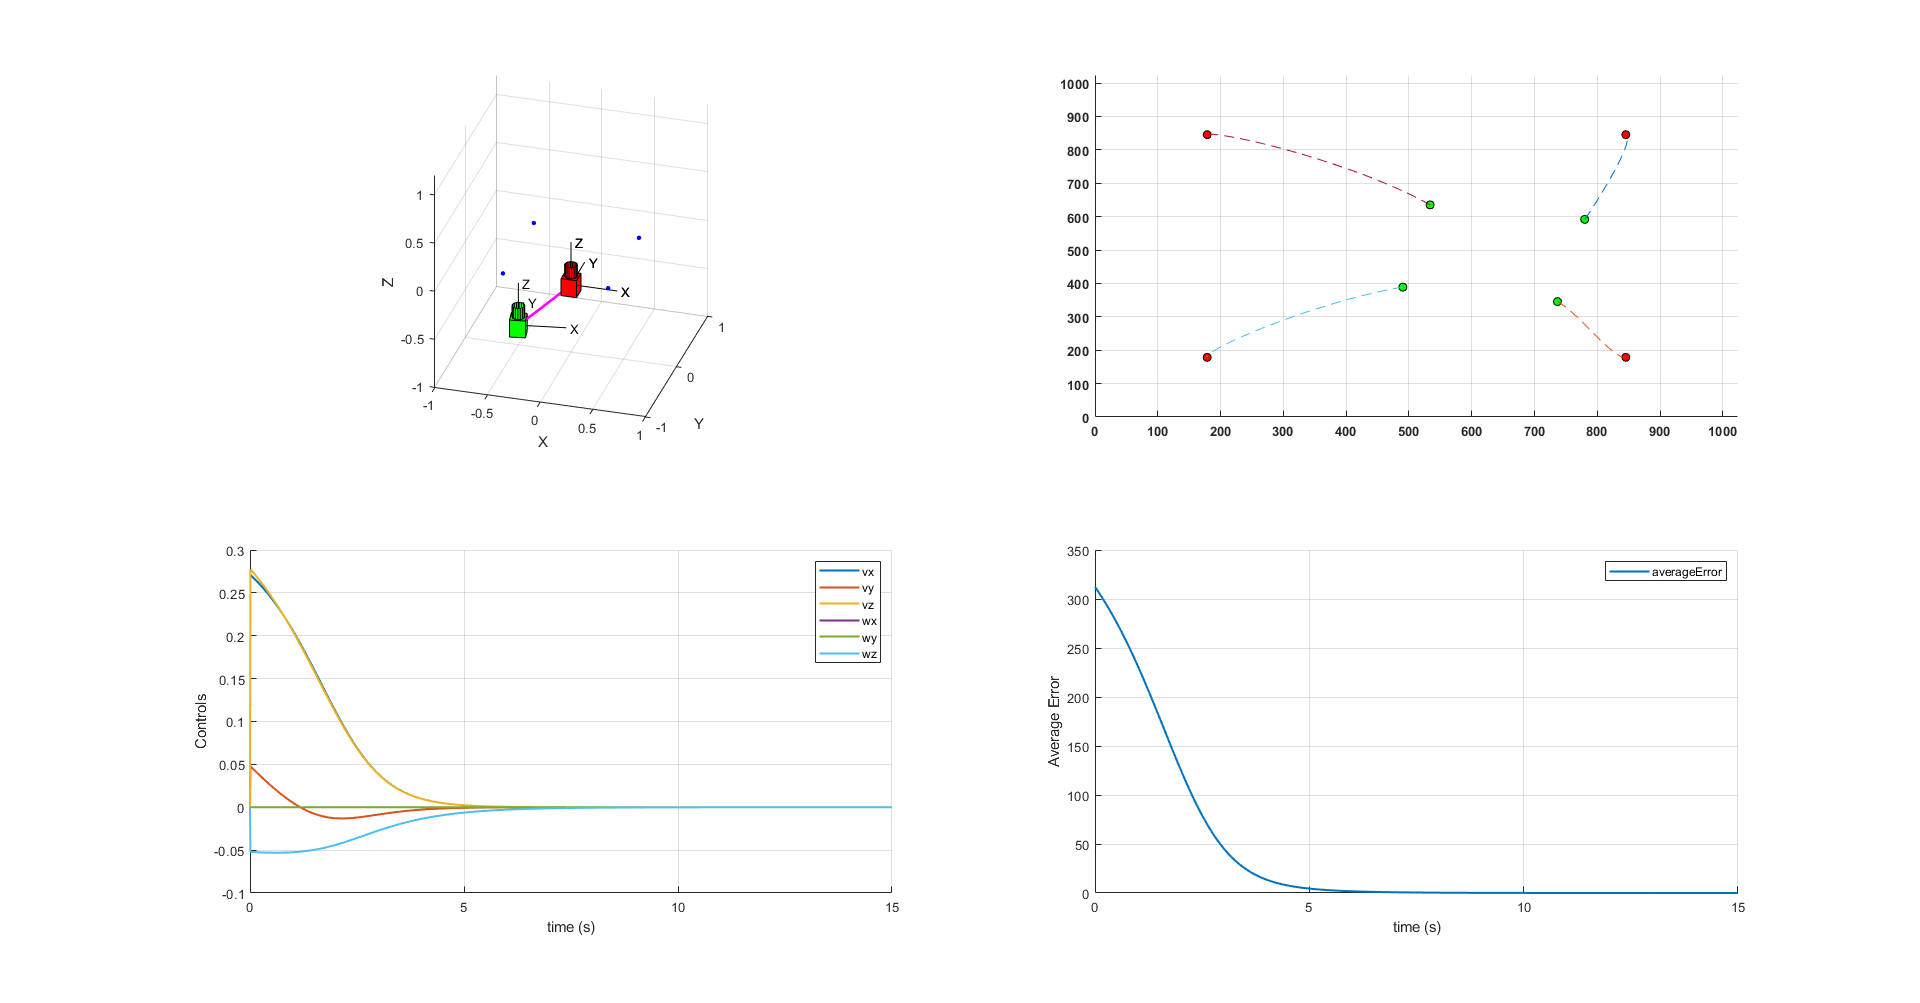
\includegraphics[scale=0.3]{fig4_3.png}\\
	{\footnotesize \textbf{Figura 10}. Subestimaci\'on de la profundidad. Con una subestimaci\'on, es decir que la profundidad es m\'as corta que la real, se logra una convergencia m\'as r\'apida a la posici\'on deseada.}\\
	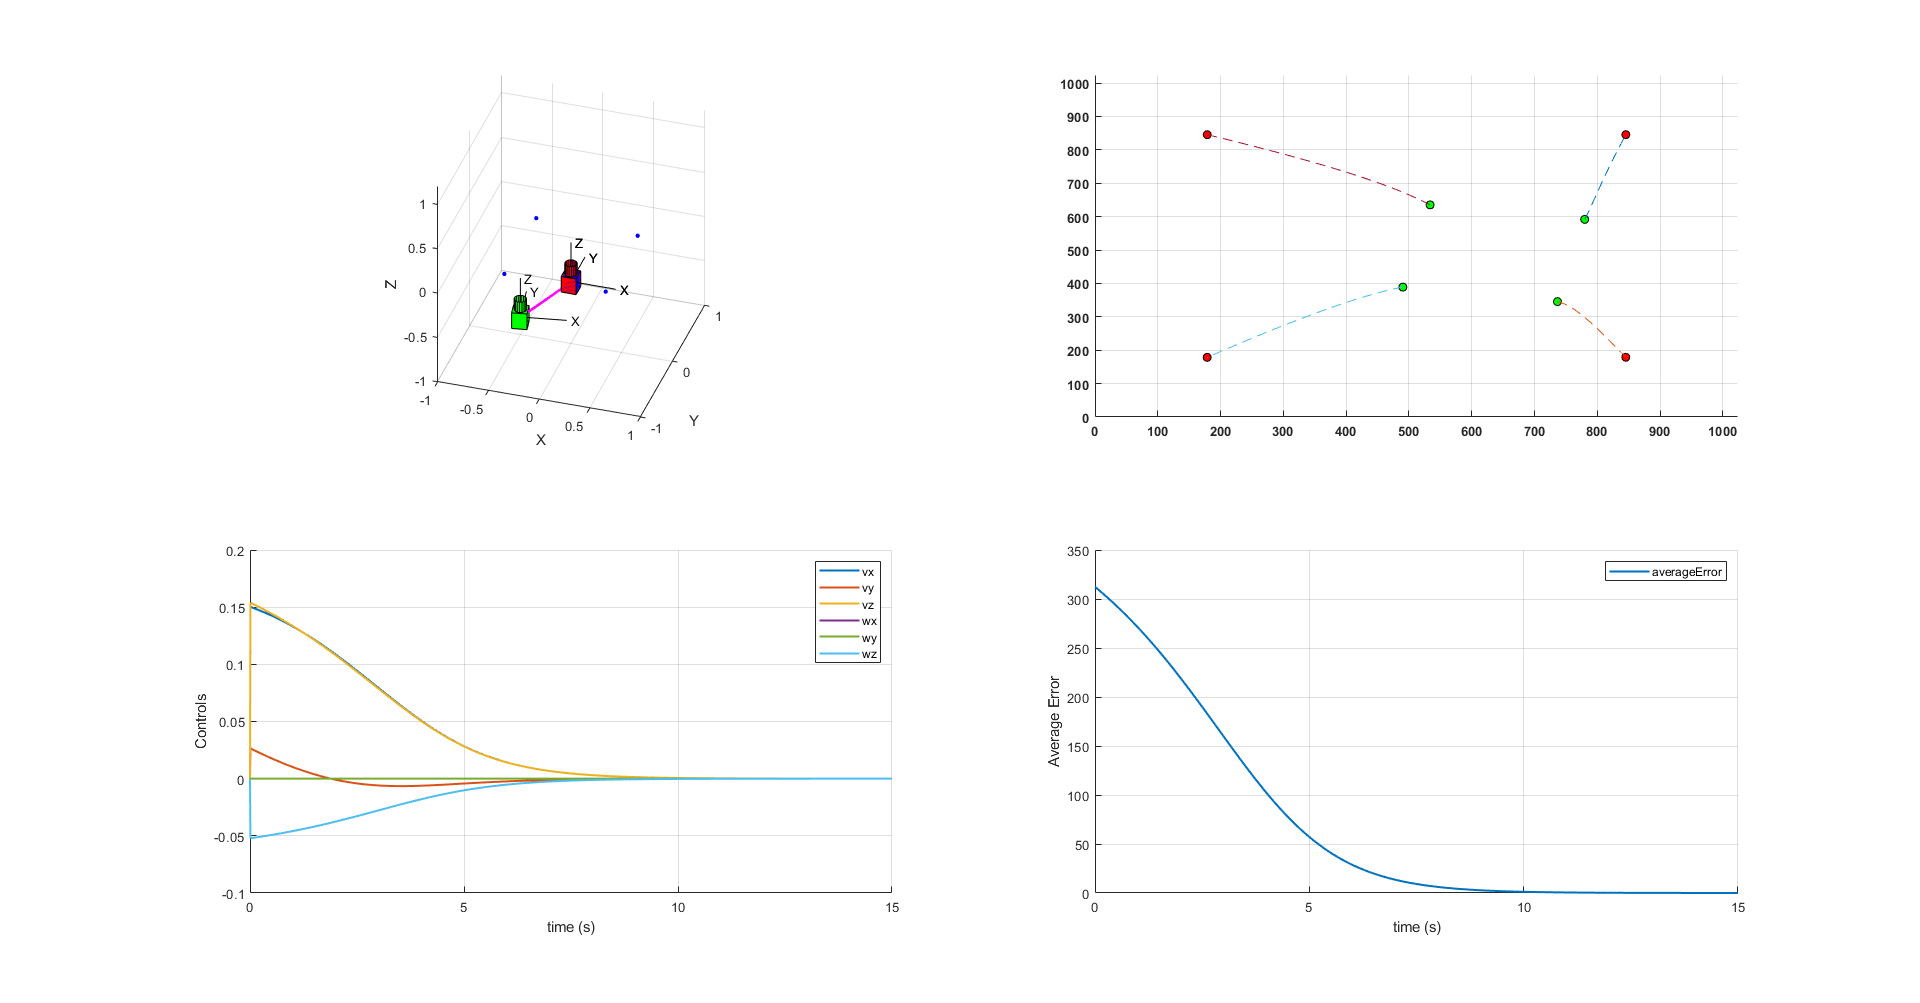
\includegraphics[scale=0.3]{fig4_2.png}\\
	{\footnotesize \textbf{Figura 11}. Estimaci\'on cercana a real. Se consiguen resultados cercanos a los obtenidos en la figura 1.}\\
	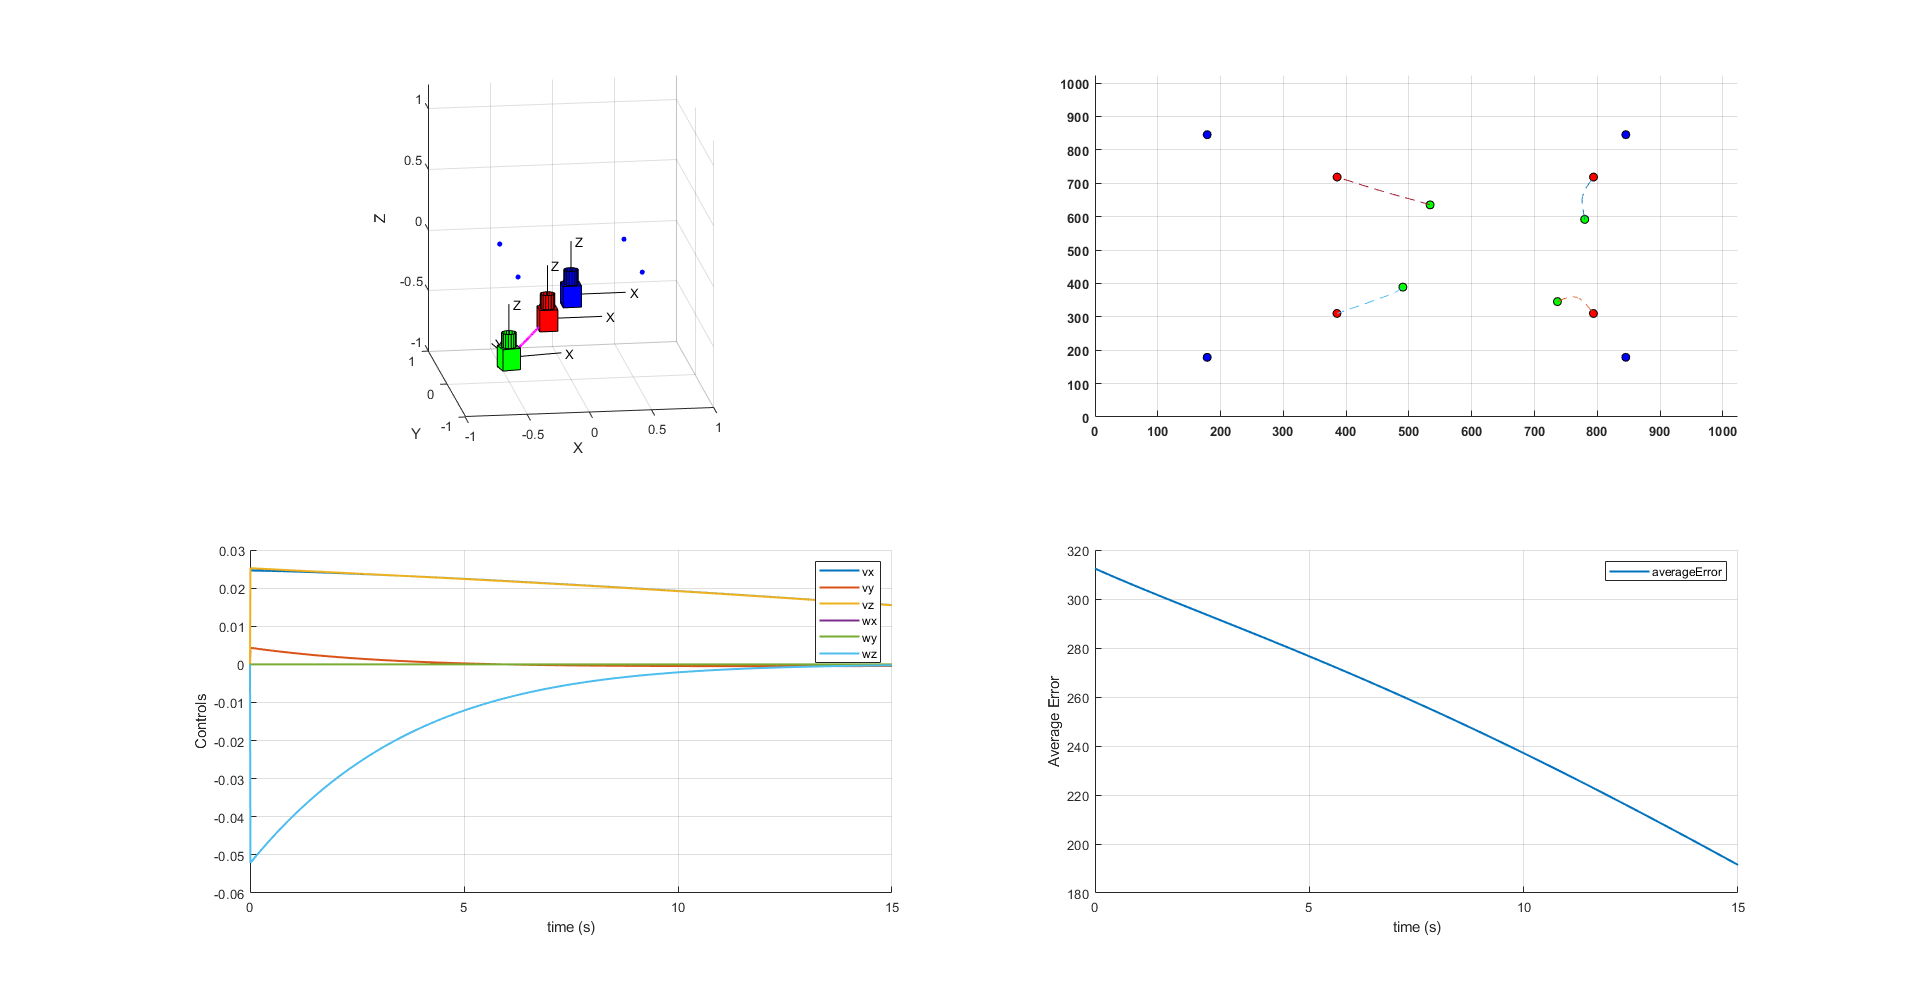
\includegraphics[scale=0.3]{fig4_1.png}\\
	{\footnotesize \textbf{Figura 12}. Sobreestimaci\'on de la profundidad. Con una sobreestimaci\'on, es decir que la profundidad es mayor que la real, la c\'amara no es capaz de llegar a la posici\'on deseada en el tiempo establecido.}\\
	\end{center}
	
	\section{Longitud focal}
	Anteriormente se hab\'ia usado un valor de longitud focal de $0.002$, a continuaci\'on se presentan los resultados para distintos valores de este par\'ametro usando los vectores de caracter\'isticas iniciales y deseadas $s_{init}$, $s_{goal}$.
	
	\begin{center}
		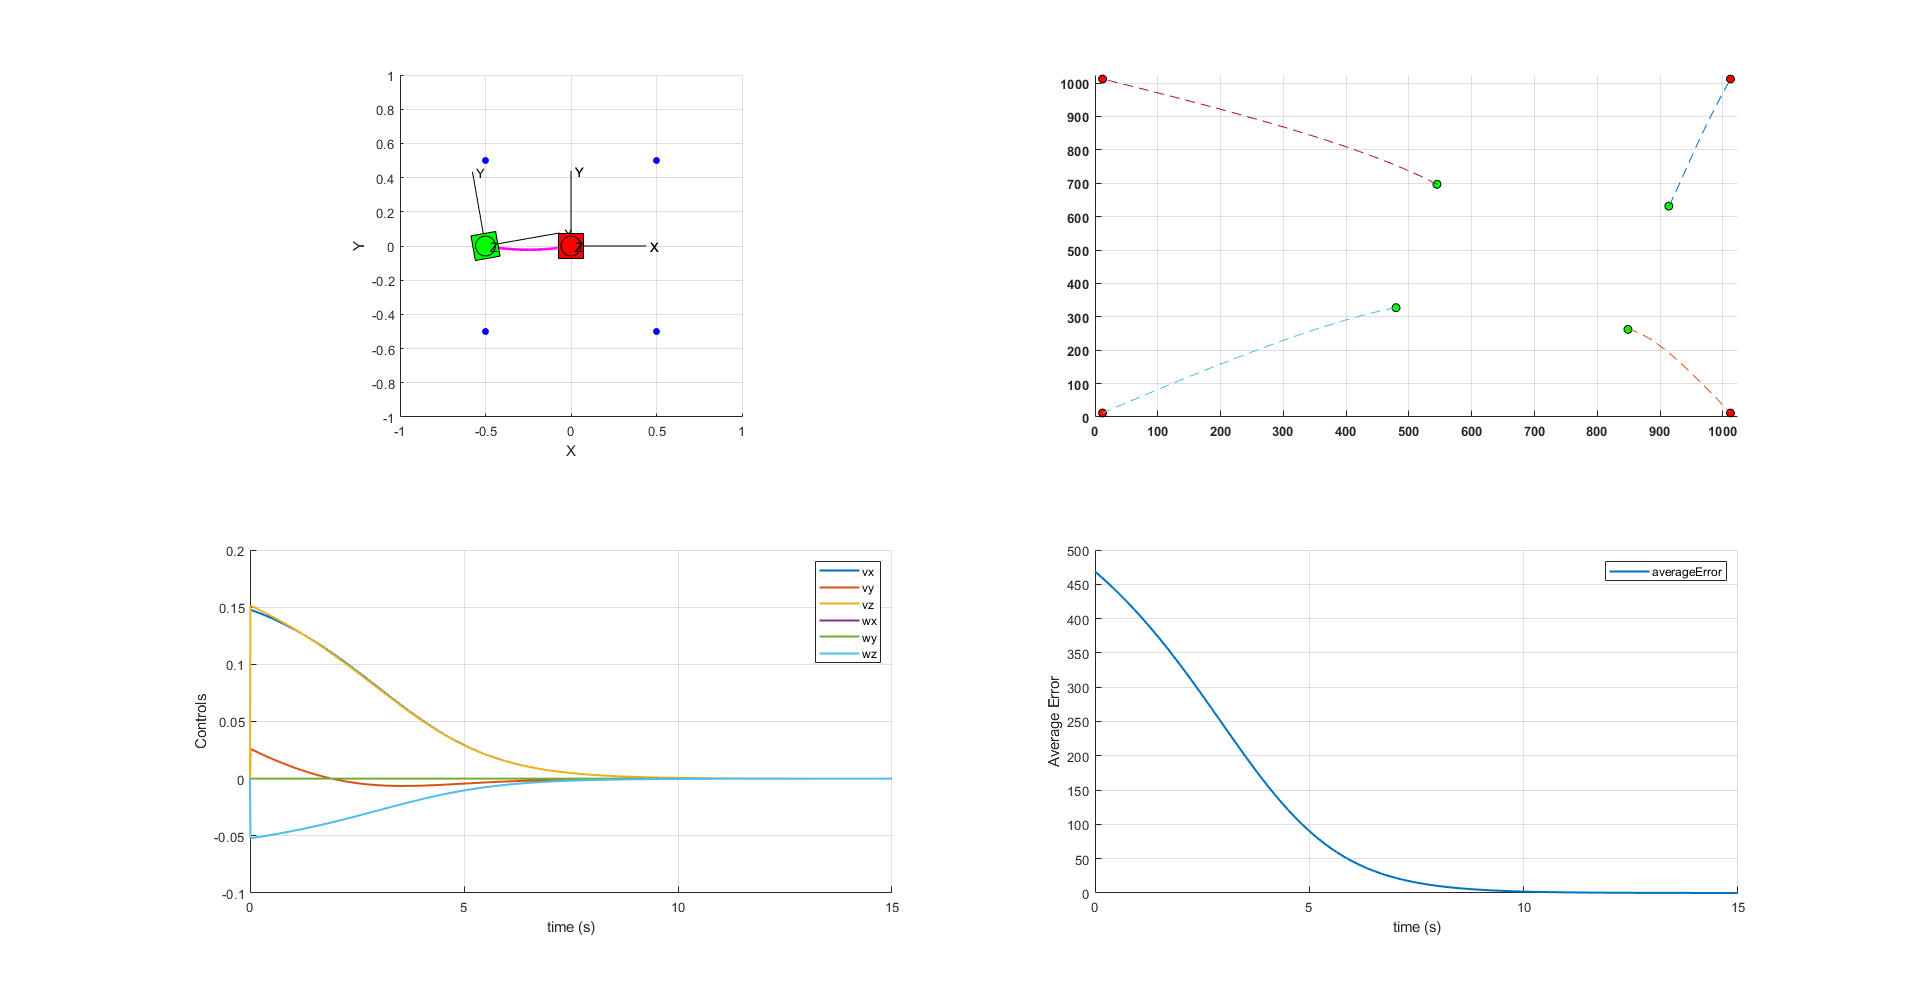
\includegraphics[scale=0.3]{fig5_1.png}\\
		{\footnotesize \textbf{Figura 13}. Resultados para un valor de longitud focal $f=0.03$.}\\
		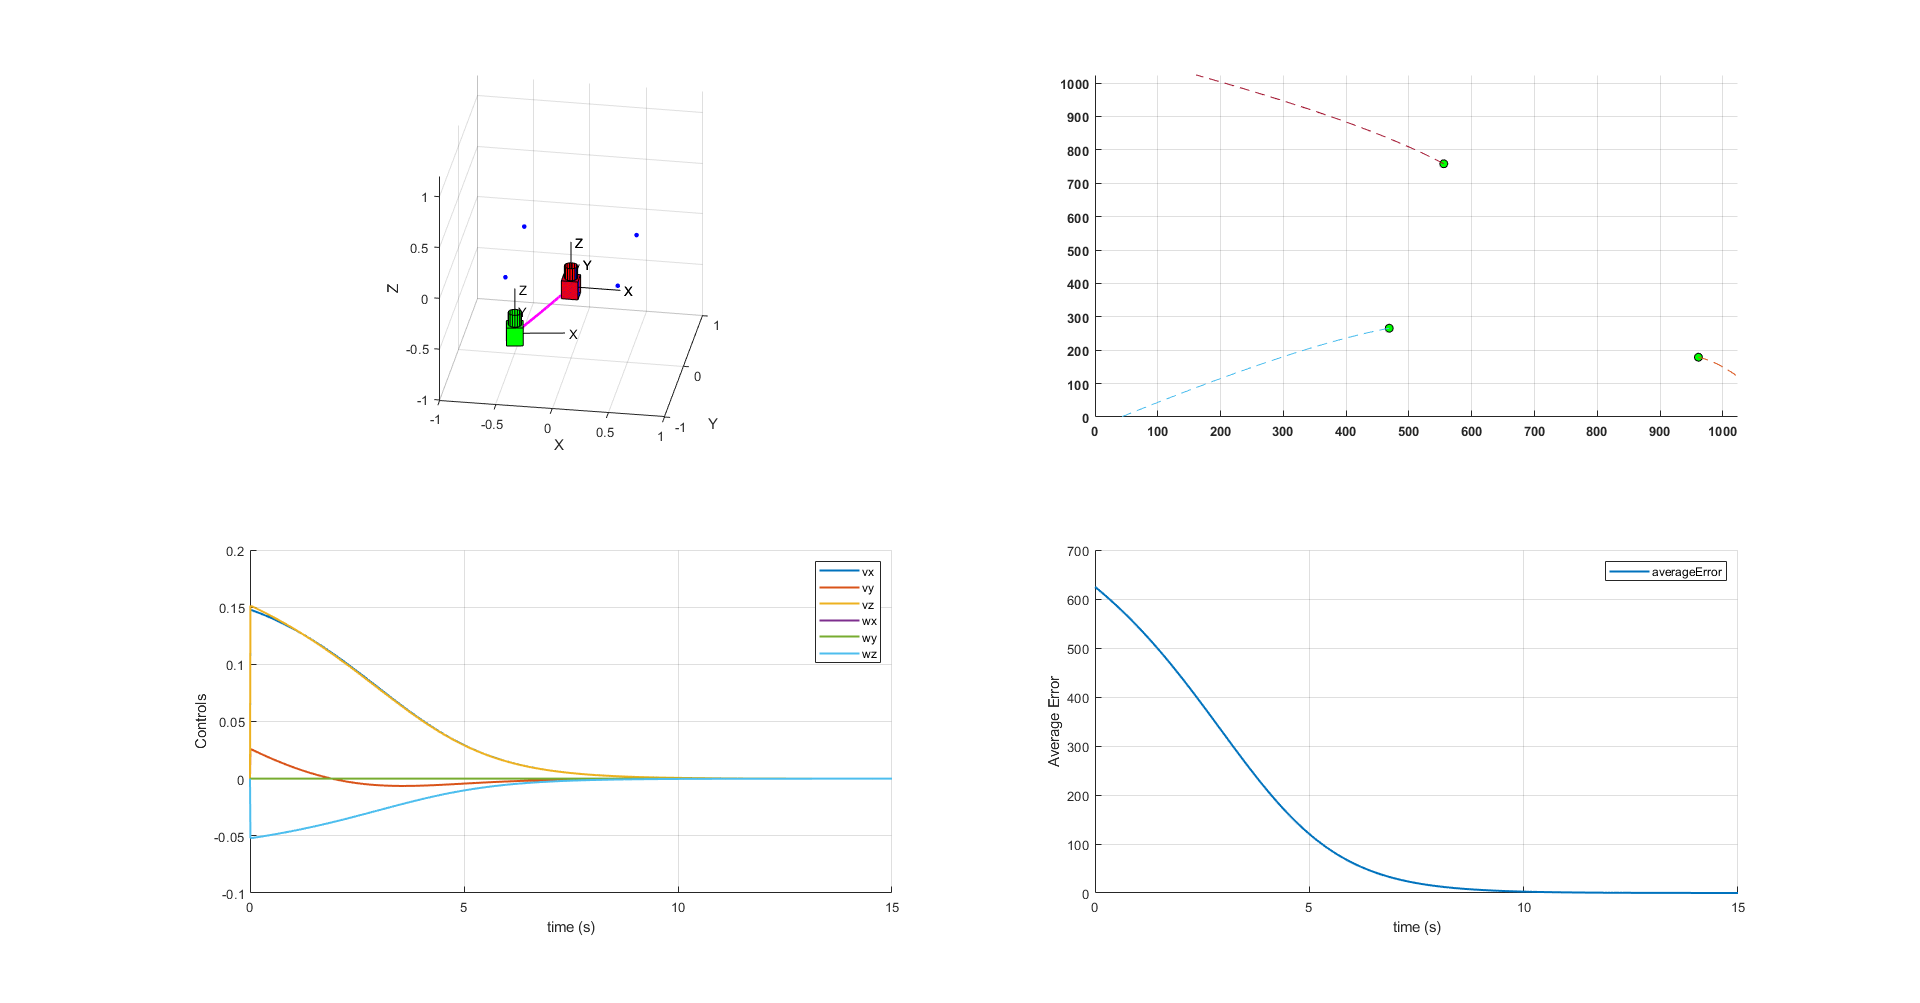
\includegraphics[scale=0.3]{fig5_2.png}\\
		{\footnotesize \textbf{Figura 14}. Resultados para un valor de longitud focal $f=0.04$.}\\
		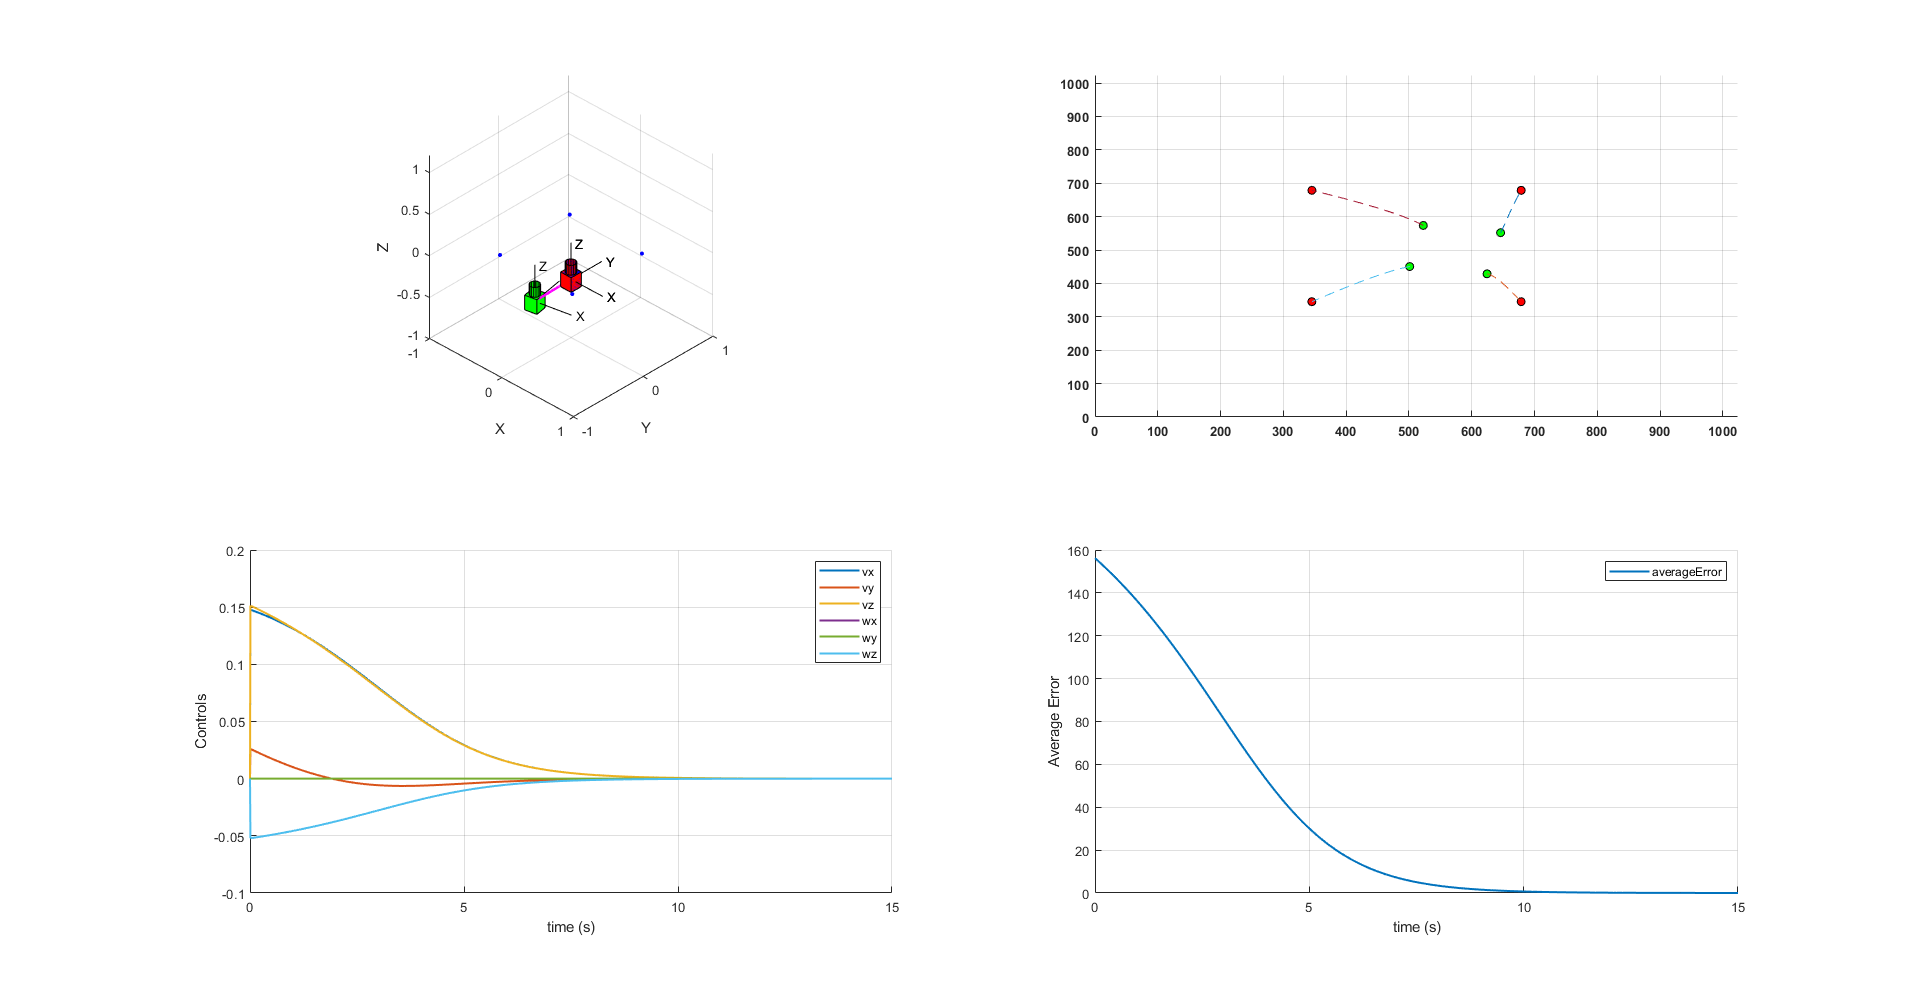
\includegraphics[scale=0.3]{fig5_3.png}\\
		{\footnotesize \textbf{Figura 15}. Resultados para un valor de longitud focal $f=0.001$.}\\
		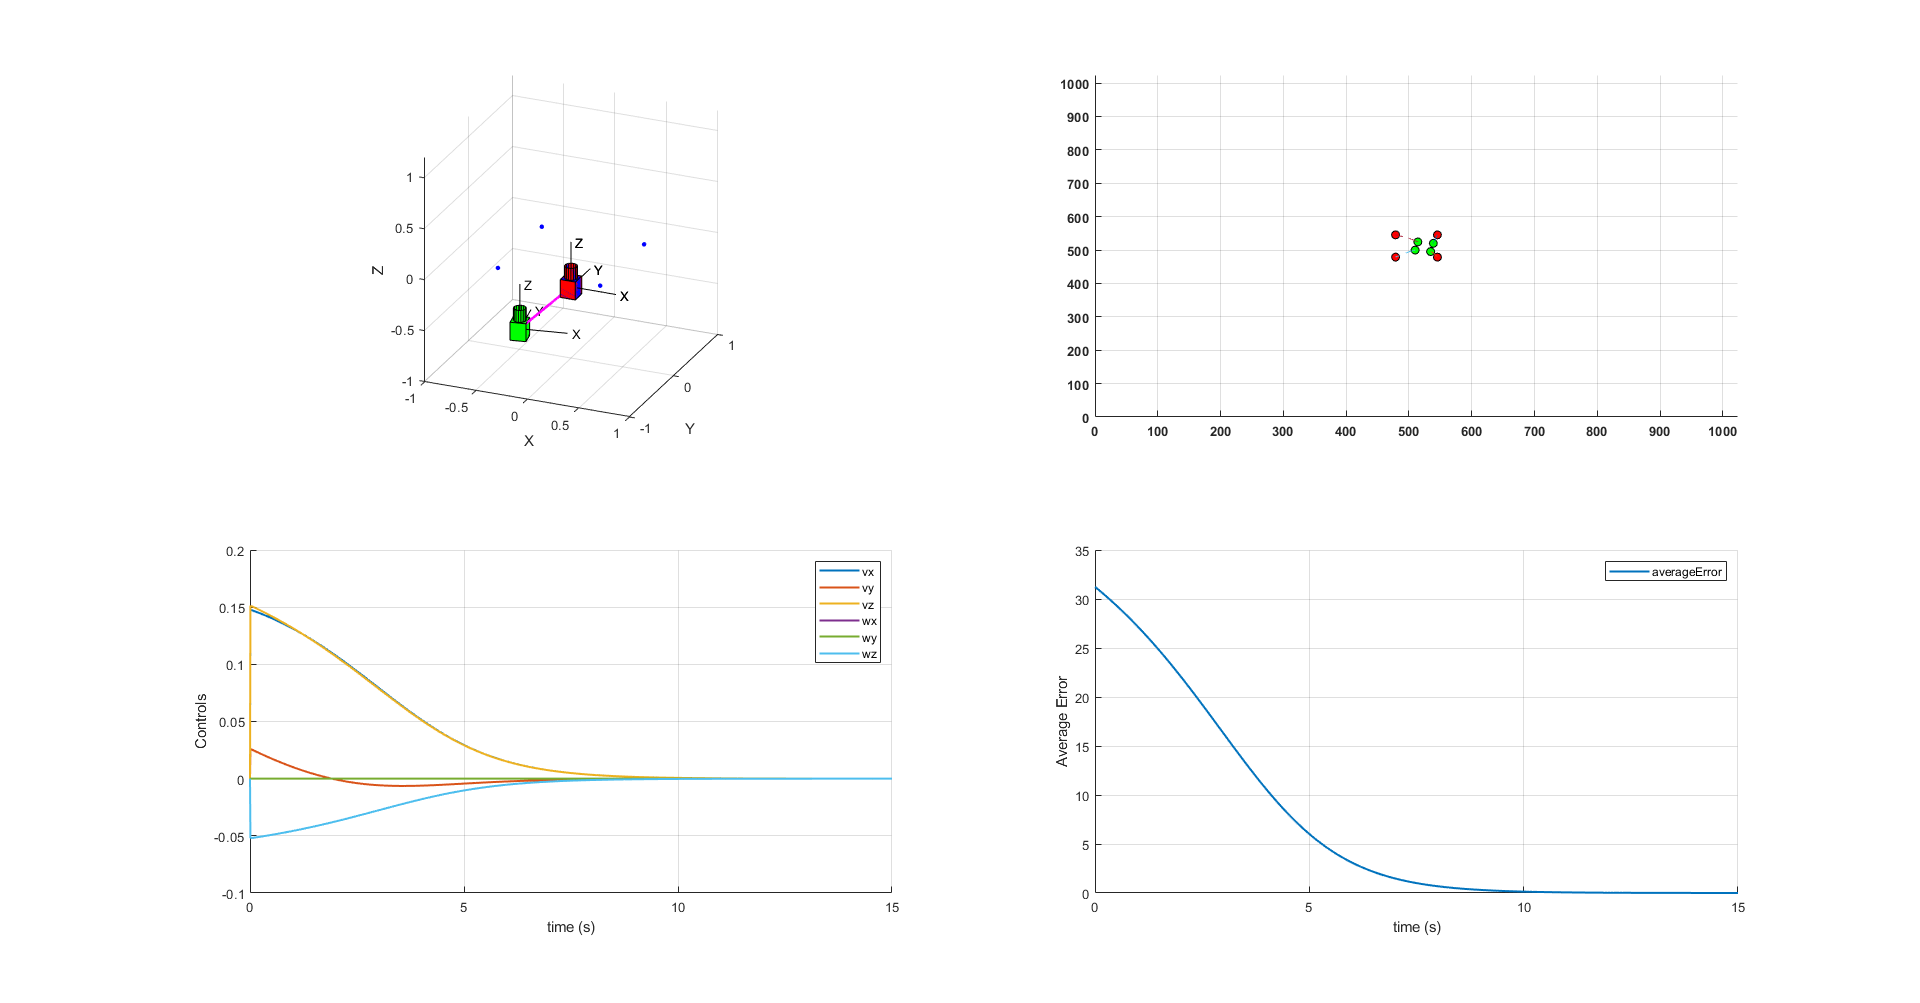
\includegraphics[scale=0.3]{fig5_4.png}\\
		{\footnotesize \textbf{Figura 16}. Resultados para un valor de longitud focal $f=0.0002$.}\\
	\end{center}
	
	La longitud focal funciona de cierta manera como una lente de zoom en la c\'amara. Se puede observar en las figuras 7 y 8 c\'omo los puntos se ven m\'as lejanos uno de otro (y por tanto la imagen parece estar m\'as cerca) ya que se escoge una longitud focal mayor a la usada con anterioridad $f>0.002$. Inclusive en la figura 8 \'estos salen del plano imagen, sin embargo es posible llevar a cabo el control en simulaci\'on ya que es posible el c\'alculo de las ubicaciones de los puntos aun fuera del plano imagen.\\
	
	De manera contraria, con valores de longitud focal menores a la usada, $f<0.002$, los puntos se ven m\'as cerca uno de otro en la imagen (haciendo que la e]imagen se vea m\'as lejos). El comportamiento de los controles en todos los casos son los mismos salvo por la gr\'afica del error promedio en la que, aunque el comportamiento y el tiempo de convergencia es el mismo en todos los casos, el total del error promedio es m\'as grande para los casos de mayor longitud focal.
	
	\section{Uso de las profundidades reales}
	Ya que se trabaja en simulaci\'on, es posible disponer de los valores reales de profundidad para los puntos en el espacio 3D. Haci\'endo uso de ellos se propone el c\'alculo del control de tal forma que en cada iteraci\'on se usen estos valores para formar y usar la matriz de iteracci\'on o jacobiano de imagen. A continuaci\'on se presentan los resultados aplicando a los vectores de caracter\'isticas iniciales $s_1$ y $s_2$, mismos a los usados en las figuras 2 y 3, tomando como vector de caracter\'isticas deseadas $s_{goal}$ como usualmente se ha usado.
	
	\begin{center}
		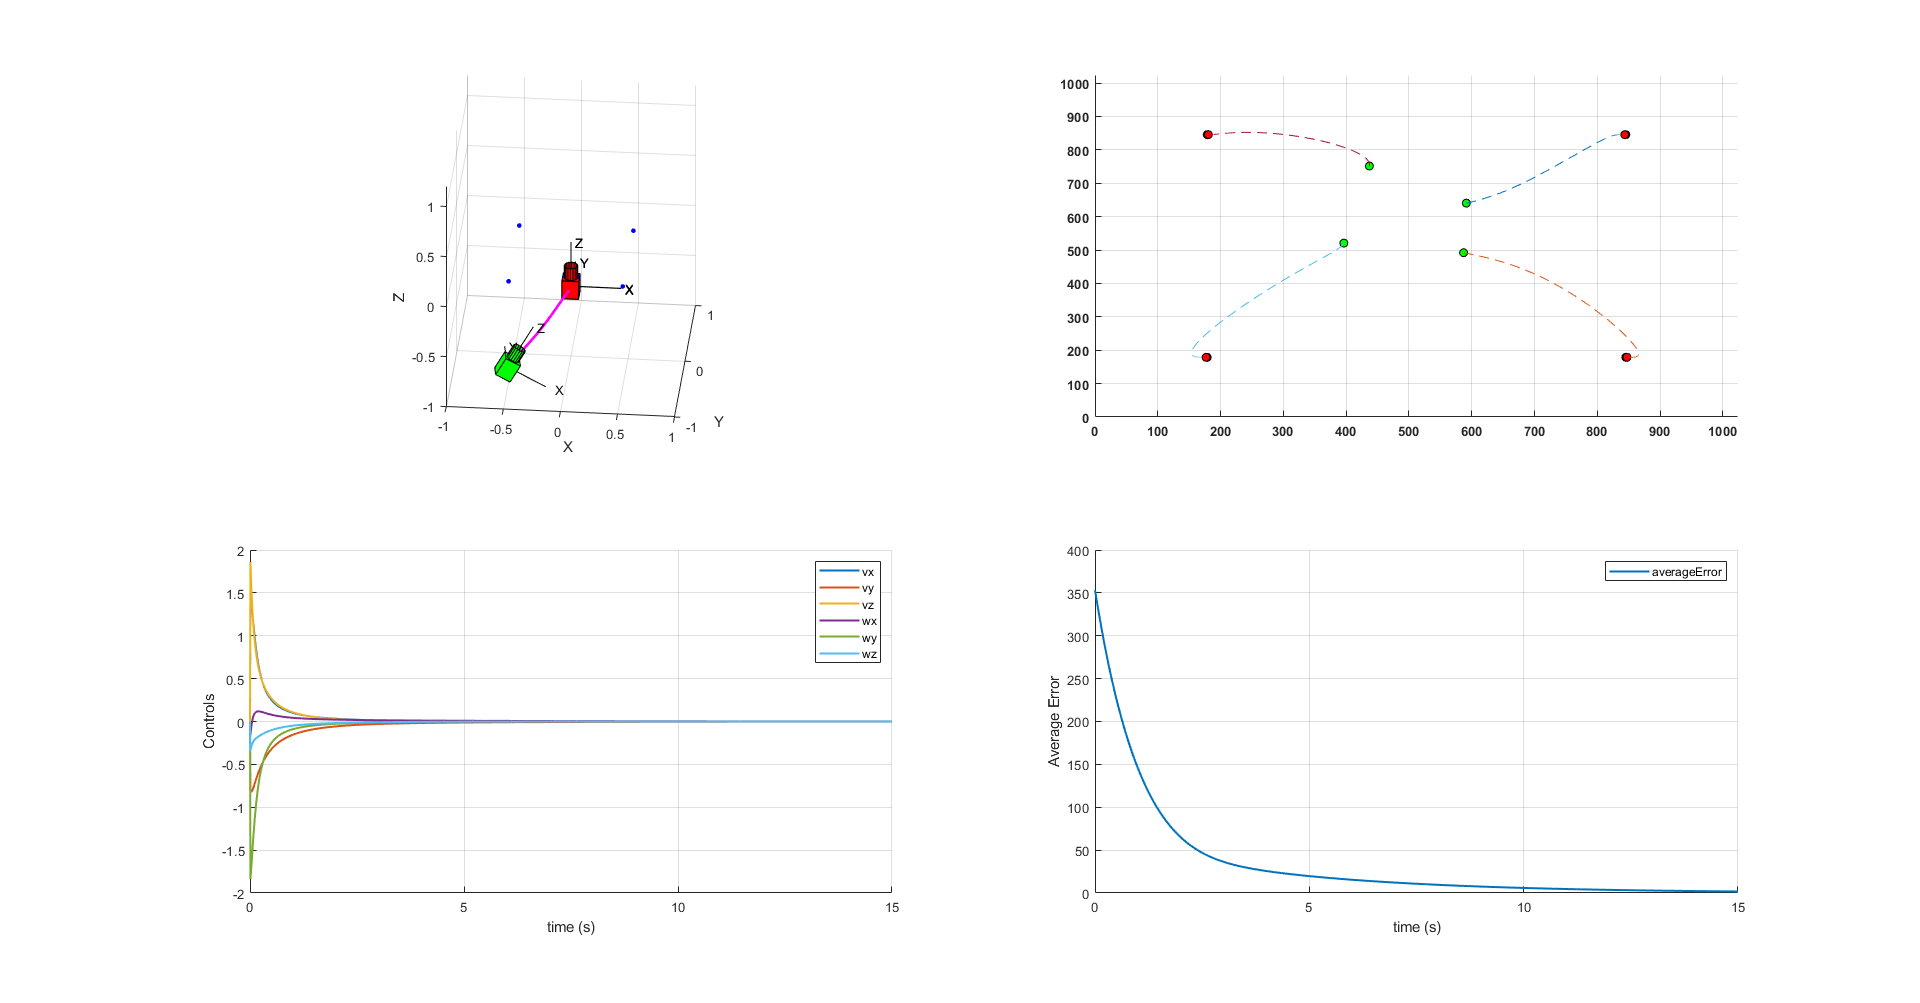
\includegraphics[scale=0.3]{fig7_1.png}\\
		{\footnotesize \textbf{Figura 17}. Resultados a partir del vector de caracter\'isticas $s_1$.}\\
		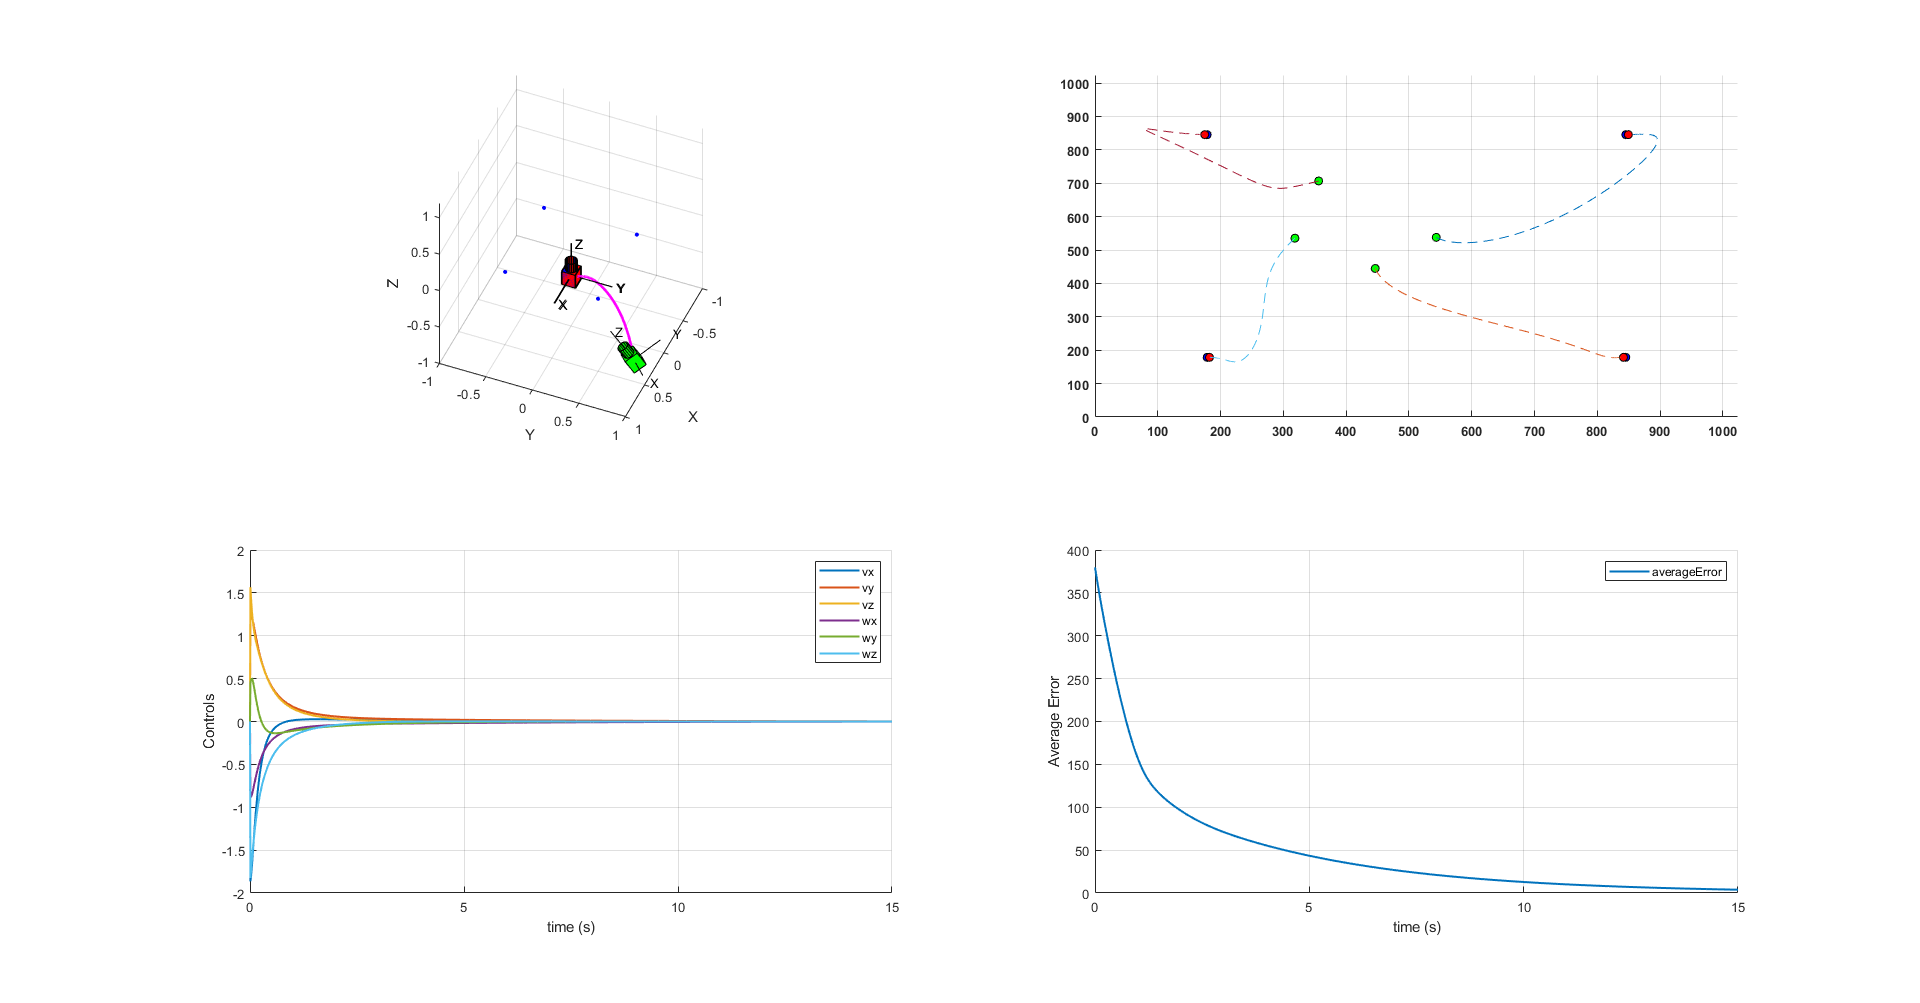
\includegraphics[scale=0.3]{fig7_2.png}\\
		{\footnotesize \textbf{Figura 18}. Resultados a partir del vector de caracter\'isticas $s_1$.}\\
	\end{center}
	
	Diferente al comportamiento registrado en las figuras 2 y 3, en las figuras 11 y 12 se mantiene un comportamiento exponencial desde el inicio de la simulaci\'on. Esto es debido a la disposici\'on del jacobiano de imagen en cada iteraci\'on a lo largo de la simulaci\'on. Cabe resaltar tambi\'en que, contrario a la figura 3, en la figura 12 la trayectoria de los puntos no salen del plano imagen.



\end{document}